%% Template for a preprint Letter or Article for submission
%% to the journal Nature.
%%

\documentclass[%
%superscriptaddress,
%groupedaddress,
%unsortedaddress,
%runinaddress,
%frontmatterverbose, 
%preprint,
showpacs,
%preprintnumbers,
%nofootinbib,
%nobibnotes,
%bibnotes,
 amsmath,amssymb,
 aps,
 twocolumn,
 prl,
 reprint,
%pra,
%prb,
%rmp,
%prstab,
%prstper,
floatfix,
]{revtex4-1}

\usepackage{graphicx}% Include figure files
\usepackage{dcolumn}% Align table columns on decimal point
\usepackage{bm}% bold math
%\usepackage{lineno}
\usepackage{color}
\usepackage{acronym}
\usepackage{multirow}
\usepackage{tabularx}
\usepackage{hyperref}

\hypersetup{
%--- fill inside borders ---
  colorlinks=true,        % false: boxed links; true: colored links
  linkcolor=black,         % color of internal links
  citecolor=cyan,         % color of links to bibliography
}

%% ----- comment commands for each of us
\newcommand{\chris}[1]{\textbf{\textcolor{red}{CHRIS: #1}}}
\newcommand{\francesco}[1]{\textbf{\textcolor{green}{FRANCESCO: #1}}}
\newcommand{\hunter}[1]{\textbf{\textcolor{blue}{HUNTER: #1}}}
\newcommand{\siong}[1]{\textbf{\textcolor{cyan}{SIONG: #1}}}
\newcommand{\rod}[1]{\textbf{\textcolor{yellow}{ROD: #1}}}

\begin{document}

\preprint{APS/123-QED}

\title{Estimating Bayesian parameter estimation using conditional variational
autoencoders for gravitational-wave astronomy}

\author{Hunter Gabbard$^1$}
 \email{Corresponding author: h.gabbard.1@research.gla.ac.uk}
\author{Chris Messenger$^1$}
\author{Ik Siong Heng$^1$}
\author{Francesco Tonolini$^2$}
\author{\& Roderick Murray-Smith$^2$}

\affiliation{
 SUPA, School of Physics and Astronomy$^1$, \\
 University of Glasgow, \\
 Glasgow G12 8QQ, United Kingdom \\ \\
 School of Computing Science$^2$, \\
 University of Glasgow, \\
 Glasgow G12 8QQ, United Kingdom \\
}

\date{\today}

\maketitle

\acrodef{GW}[GW]{gravi	tational wave}
\acrodef{BBH}[BBH]{binary black hole}
\acrodef{SNR}[SNR]{signal-to-noise ratio}
\acrodef{PSD}[PSD]{power spectral density}
\acrodef{FFT}[FFT]{fast Fourier transform}
\acrodef{CNN}[CNN]{convolutional neural network}
\acrodef{ROC}[ROC]{receiver operator characteristic}
\acrodef{ELBO}[ELBO]{evidence lower bound}
\acrodef{LIGO}[LIGO]{advanced Laser Interferometer Gravitational wave Observatory}
\acrodef{CVAE}[CVAE]{conditional variational autoencoder}
\acrodef{AD}[AD]{Anderson-Darling}
\acrodef{KS}[KS]{Kolmogorov-Smirnoff}
\acrodef{KL}[KL]{Kullback–Leibler}

%
% Introductory paragraph describing the content of the letter
%
% This format begins with a title of, at most, 15 words, followed by an
% introductory paragraph (not abstract) of approximately 150 words, summarizing
% the background, rationale, main results (introduced by "Here we show" or some
% equivalent phrase) and implications of the study. This paragraph should be
% referenced, as in Nature style, and should be considered part of the main
% text, so that any subsequent introductory material avoids too much redundancy
% with the introductory paragraph.
%
\textbf{ 
%
% background
%
With the beginning of the \ac{LIGO} and
Virgo's third observation run well under way, we are now in an era where
\ac{GW} detection is commonplace~\cite{PhysRevLett.116.061102,
PhysRevX.6.041015,PhysRevLett.119.161101}. As the sensitivity of both detectors
increases, we will see upwards of 100s of \ac{GW} events per year \cite{1409.7215}.  The current
method used to estimate the parameters of gravitational wave events is done
using Bayesian inference~\cite{1409.7215}.
%
% rationale
%
Bayesian inference has been shown to be incredibly effective when 
applied towards \ac{GW} parameter estimation. It is also computationally expensive 
to run. When run on a single \ac{BBH} signal sampled at 4kHz, Bayesian 
inference can take $\mathcal{O}(1.5\textrm{e}5 - 1.7\textrm{e}6\: s)$ to complete \cite{1409.7215}. 
Over the next several years, as the detectors become more sensitive, we will 
need to be able to alert our electromagnetic follow-up partners in a timely 
and efficient manner. The current fastest method for doing so, \texttt{Bayestar}, 
takes $\mathcal{O}(1\: \textrm{minute})$ to produce fast, but only approximate parameter estimates. 
Given the deluge of signals we are expecting to see, 
it is imperative that a more efficient low latency parameter estimation 
method be developed. We propose the use of a \ac{CVAE} as a rapid and accurate alternative to this
approach~\cite{1904.06264,1812.04405}. 
%
% results
%
Here we show that a machine learning algorithm can return
posterior estimates on 4 parameters (this may be extended up to 15 parameters) of a detected \ac{GW} event on the order of less
than $1s$~\chris{we need to measure this number.}, a 6 order of magnitude speed-up over
current inference techniques.}

\chris{
The paragraph structure needs to be changed a bit. Here's how I see it based on
this text from the Nature guidelines - "As a guideline, the text should be
structured in broad sections (abstract, introduction, results, conclusions,
methods)." 
\begin{itemize} 
%
\item Abstract - introductory paragraph
(not abstract) of approximately 150 words, summarizing the background,
rationale, main results (introduced by "Here we show" or some equivalent
phrase) and implications of the study. It's getting there.  
%
\item introduction - this section has to expand upon what has mentioned in the
abstract background (which was only ~50 words). It needs to cover the state of
the gravitational wave field and the number of detections expected in the next
~5 years. It should briefly discuss the issue of low latency EM follow up. It
needs to cover Bayesian inference (not in too much detail) and the signal model
we are interested in here (again, not too much detail but enough for the
average Nature reader). It then needs to introduce machine learning and focus
mainly on how our scheme works. We also need to include a statement about how
the training data priors affect the result (are they really the priors?)   
%
\item results - here you would outline the process of comparison between the
standard approach and the new one. Define training and test data and how Bilby
is run on all test data for comparison. How do we then train our network. How
do we then produce results on the test data. Here you refer to results plots
but try to not make conclusion statememnts (just descriptive). Also include the
speed analysis here.  
%
\item conclusions - now draw conclusions about the quality of the comparison
results. Highlight the current limitations but also highlight the importance of
this for the GW field (multi-detector is easy, additional parameters are easy,
longer datasets may be a challenge regarding GPU memory?, we don't have to
assume a noise model if we inject training data into real noise, we do rely on
well defined signal models, EM-follow up in very low latency, can we use
transfer learning if we want to retrain, ...) End with broader statements about
inference in other fields and how this is applicable across the sciences.
%
\item methods - Everything that we couldn't fit in. Mostly validation plots.
%
\end{itemize} }

%%%%%%%%%%%%%%%%%%%%%%%%%%%%%%%%%%%%%%%%%%%%%%%%%%%%%%%%%%%%%%%%%%%%%%
% INTRODUCTION
%%%%%%%%%%%%%%%%%%%%%%%%%%%%%%%%%%%%%%%%%%%%%%%%%%%%%%%%%%%%%%%%%%%%%%
%
% Intro to the detection era with the LVC
%
With the overwhelmingly successful observation runs of O1 and O2 
now complete, \ac{LIGO} and Virgo have produced a large 
catalogue of \ac{GW} data covering both \ac{BBH} and {BNS} signals\cite{1811.12907}. Over the next five years 
we expect the number of detections to increase to be upwards 
of $\sim180$ BNS and $\sim400$ BBH events per year \cite{1304.0670,1811.12907}. This large influx in the number 
of detections will put an increased amount of pressure on the current \ac{GW} inference 
methods used for parameter estimation.  

%
% From GW detection, to parameter estimation
%
Much of the \ac{LIGO} analysis effort over the past several years has been focused 
on the detection of \ac{GW}s. This has been the primary 
focus of many, due to the difficulty associated 
with identifying \ac{GW} waveforms buried in 
in large amount of noise to a high degree of certainty. The detection problem has largely 
been solved through the use of matched template filtering\cite{0264-9381-33-21-215004}. 
Once a \ac{GW} has been identified through matched template filtering, Bayesian inference 
is used to extract information about the source 
parameters of the detected \ac{GW} event.

%
% Set up parameter estimation problem
%
In the standard Bayesian \ac{GW} inference approach, we assume that we are
given both a signal model and a noise model. Both the signal and the 
noise model may have unknown parameters we are interested in inferring. 
Each parameter is given a prior astrophysically motivated probability 
distribution. In our case, we have additive noise which is modelled as 
a Gaussian (in reality, the data is not truly Gaussian). Given a noisy
\ac{GW} waveform, we would like to find an optimal procedure for retrieving
some finite set of unknown GW parameters. Our procedure should be able
to give us an accurate estimate of the parameters of our observed signal, while
also accounting for the uncertainty which arises from having multiple noise
realizations of our observed data able to be mapped to one parameter
estimate.

%
% Describe Bayes Theorem
%
According to Bayes Theorem, a posterior for a set of GW parameters can be described by the
following expression:
%
\begin{equation}
    p(x|y) = \frac{p(y|x) p(x)}{p(y)},\label{eq:bayes_theorem}
\end{equation}
%
where $x$ are the parameters, $y$ is the
observed data, $p(x|y)$ is the posterior, $p(y|x)$ is the likelihood, $p(x)$ is
the prior we put on our parameter distribution and $p(y)$ is the probability of
our data, known as the Bayesian evidence or the marginal likelihood. We
typically ignore $p(y)$ since the term is a constant and we are only interested
in the shape of the posterior distribution, not its normalization. Eq.
\ref{eq:bayes_theorem} then reduces to
%
\begin{equation}\label{eq:simplified_bayes} 
p(x|y) \propto p(y|x) p(x).
\end{equation} 
   
%
% Intro to machine learning section
%
Machine learning has featured prominently in many areas of gravitational wave
research over the last few years. These techniques have shown to be
particularly promising in signal detection
\cite{GEORGE201864,PhysRevLett.120.141103,1904.08693}, glitch classification
\cite{1706.07446,0264-9381-34-6-064003} and earthquake prediction
\cite{Coughlin_2017}. Recently, a type of neural network called conditional
variational autoencoders was shown to perform exceptionally well when applied
towards computational imaging inference~\cite{1904.06264,NIPS2015_5775}, text
to image inference \cite{1512.00570}, high-resolution synthetic image
generation \cite{1612.00005} and the fitting of incomplete heterogeneous data
\cite{1807.03653}. It is this type of machine learning network that 
we will utilize to reproduce the Bayesian posterior, which is known to be 
the optimal result.

%
% What is an autoencoder?
%
Conditional variational autoencoders are a form of variational autoencoder
which are conditioned on an observation, where in our case the observation is a
\ac{GW} 1-dimensional time series signal $y$. The autoencoders from which
variational autoencoders are derived are typically used for problems involving
image reconstruction and/or dimensionality reduction. They essentially perform
a regression task whereby the autoencoder tries to predict its own given input
(model the identity function) through a limited distilled version of the input 
parameter space. An autoencoder is composed of two neural networks, an encoder and a decoder~\cite{LIOU20083150}. The encoder network takes as input an
$n$-dimensional vector, where the number of dimensions is a fixed number
predefined by the user. The encoder converts the input $n$-dimensional vector into a (typically) lower dimensional space, what is also known as the {\it{latent space}}. A
representation of the data in the latent space is passed to the decoder network
which generates a reconstruction of the original input data to the encoder
network. Through training, we learn a how to efficiently represent 
a dataset within a lower dimensional latent space which will take on the most important properties of our input training samples. When applying an autoencoder to some
input data, one hopes that the data can be represented in a latent space
smaller than the dimensionality of the input data.  In this way, the data can
be compressed with little loss of fidelity. Training continues by passing 
the learned latent space from the encoder to the decoder network, 
whereby the decoder tries to predict the input data given initially 
to the encoder network. The decoder then learns to decode or reconstruct the latent space back to its original form (the input data). 

%
% What is a variational autoencoder?
%
%Autoencoders, once trained, represent a deterministic algorithm which maps
%only one given input to one output. If we would like to produce multiple
%variable estimates for one given input, we need to utilize a variational
%autoencoder~\cite{1812.04405}
A variational autoencoder ~\cite{1812.04405} is also composed of both an
encoder and a decoder network. The primary difference between a variational
autoencoder and an autoencoder concerns the method by which the latent space is
produced. In our variant of the variational autoender, the first two central 
moments of the encoder output distribution are calculated ($\mu$). These are
interpreted as parameters governing statistical distributions (in our case the
means and variances of multivariant Gaussians). In proceeding to the decoder
network, samples are drawn from these distributions ($z$) and fed into the
decoder, therefore adding an element of variation into the process.  Thus a
particular input can have infinitely many outputs. In both the decoder and the
encoder networks we use fully-connected layers (although this is not a
constraint, any trainable network architecture may be used).

% latent space expression
%\begin{equation}
%    z = z_{\mu} + z_{\log{(\sigma^{2})}} \cdot \epsilon(0,1).\label{eq:z_calc}
%\end{equation}

%
% Brief introduction to loss functions used in the neural networks
%
We wish to be able to make a numerical function that can
simulate a target distribution (the posterior for \ac{GW} parameters). This is done through a 
combination of three fully-connected networks; two encoder networks ($\textrm{E}_1$,
$\textrm{E}_2$) and one decoder network (D) (see Fig.
\ref{fig:network_config}). In order for our variational autoencoders to learn anything, we need a metric by which 
we can assess the effectiveness of our three networks. We therefore start with a cross-entropy which minimizes the difference between predicted samples from the posterior with respect to the truth and we then arrive at a cost function 
(see the methods section). We additionally minimize the Kullback-Leibler divergence 
between latent space distributions from $\textrm{E}_1$ ($z_1$) and 
$\textrm{E}_2$ ($z_2$). 

\begin{figure}
    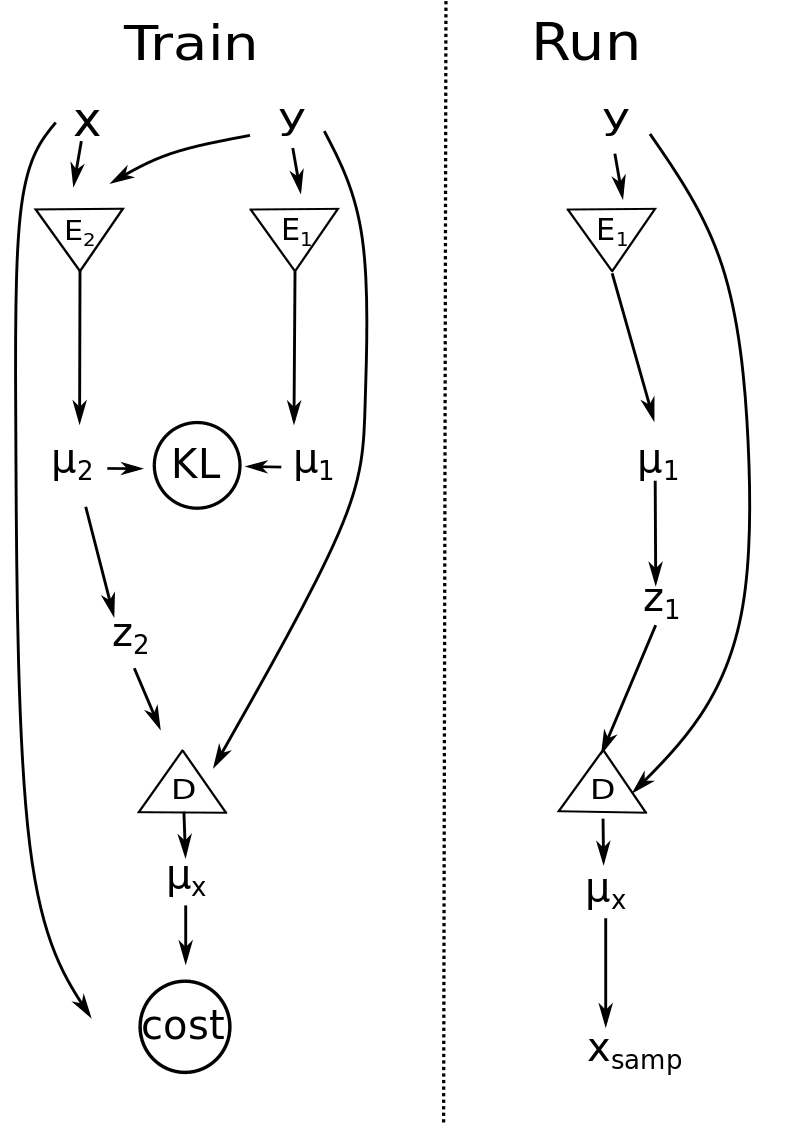
\includegraphics[width=\columnwidth]{images/network_setup.png}
    \caption{\label{fig:network_config}\chris{Why have we made it so encoder 1 is on the right and encoder 2
is on the left. It reads weird.} This figure illustrates our neural network
training/testing operations. During training, a training set of GW signals
($y$) and their corresponding true parameters ($x$) are given as input to
encoder networks $\textrm{E}_1$ and $\textrm{E}_2$. The KL divergence (Eq.
\ref{eq:kl}) is computed between the moments of latent space predictions from both
encoder networks ($\mu^{j}_{1},\mu^{j}_{2}$). We then sample from a multivariate Gaussian whose mean and variances are defined by $\mu^{j}_{2}$. These samples are given as input to the decoder network. We take the first two moments $\mu^{j}_x$ of the predictions 
from the decoder network, along with our training parameters $x$ and compute a cost function Eq. \ref{eq:cost}. After having trained our networks, we
test using only $\textrm{E}_1$ and the decoder. Using the $\textrm{E}_1$ encoder (which is similar to $\textrm{E}_2$ but uses only $y$ data input) latent space 
predictions are given to the decoder which returns an output. This output represents the parameters of the mult-dimensional Gaussian function
that describes the likelihood/posterior and so we simply sample from it. We 
then have a generated set of posterior samples.} 
\end{figure}

%
% Training procedure
%
Training is performed through a series of several
steps illustrated in Fig.~\ref{fig:network_config}. Encoder $\textrm{E}_1$ is given a set of training \ac{GW}
signals ($y$) and encodes $y$ into latent space
$\mu^{j}_{1}$, where $\mu^{j}_{1}$ is composed of the first 2 central moments for 
each dimension of a multivariate Gaussian and $j$ is the order of the moment 
($j=1$ is the mean and $j=2$ is the variance). Encoder $\textrm{E}_2$ takes a combination of $(x,y)$ and is
encoded into a latent space described by $\mu^{j}_{2}$.  We then sample
from a multivariate Gaussian distribution whose mean and standard deviation are
described by $\mu^{j}_{2}$. These samples, along with $y$, then go to
the decoder in order to get out a statistical description of another
multivariate Gaussian distribution ($\mu^{1}_x$). A cost function is then
computed between $\mu^{1}_x$ and the corresponding training parameters
($x$) and is minimized.  Essentially, the cost function is used to learn how
to predict the closest value of $x$ (through $\mu^{1}_x$) and the variation of
that $x$ (through $\mu^{2}_x$). \ac{GW} Parameter predictions $\mu^{1}_x$ and $\mu^{2}_x$ are not fixed for the whole
dataset - so they're not modelling the spread of $x$ as a multivariate Gaussian
- they have learned the $\mu^{1}_x$ and $\mu^{2}_x$ for any input pair of $x$
  and (crucially) $y$. Additionally, the K-L divergence between the 
  distributions described by $\mu^{j}_1$ and $\mu^{j}_2$ is computed and minimized in order to ensure that both distributions are
consistent with each other. For further details on training and the full 
derivation of the loss functions, see methods subsection \textit{Loss function derivation}.

%
% Cost function
%
%The cost function is constructed by first defining a normalization
%factor\chris{it's not really the first thing we have to understand though is
%it. It's just the first thing that gets computed. Try to draw a distinction
%between the functions that we have to compute and the specific ways in which
%they are implemented in the code. The reader does not care about the latter.}
%
%\begin{equation}
%    f_{\textrm{norm}} = 0.5 \log(c + \exp(x_{\sigma})) - 0.5 \log(2\pi),
%\end{equation}
%
%where $c$ is a small constant~\chris{things like the small constant are not
%important for understanding how this all works so I wouldn't mention it at all.}
%and $x_{\sigma}$ are standard deviation predictions on the source paramters
%from the decoder network given latent space predictions from encoder-2
%($z_2$\chris{be careful with what you call things.  The latent space
%predictions from encoder 2 are actually means and variances NOT the random
%draws from the latent space.}) and training GW sigals ($y_{t}$). We then
%compute 
%
%\begin{equation}
%    x_{\textrm{diff}} = (x^{z,y}_{\mu} - x_{\textrm{train}})^{2},
%\end{equation}
%
%\chris{again, this is just part of the cost calculation and the reader doesn't
%need to know how it's broken up in the code.} where $x^{z,y}_{\mu}$ are the
%predicted mean parameters from the decoder network and
%$x_{\textrm{train}}$~\chris{notation consistency. Is it $x$, $x_t$ or
%$x_{\text{train}}$? I recokon just $x$.} are the true training parameters we
%are trying to predict. A Gaussian likelihood is computed and summed~\chris{OK,
%not quite true and probably my fault for saying that it was. The whole thing is
%just how it's derived from the starting point (the cross-entropy) and we maybe
%shouldn't read more into it.} over
%
%\begin{equation}
%    \textrm{cost} = - \sum (-\frac{x_{\textrm{diff}}}{2c  
%    x^{z^{x,y_{\textrm{train}}}_{\sigma},y_{\textrm{train}}}_{\sigma^{2}}} + %f_{\textrm{norm}}),\label{eq:cost}
%\end{equation}
%
%\chris{OK, so I think the last 3 equations can go. However, for reference, try
%to set the correct parenthesis sizes using "\\left" and "\\right" and get rid of
%the "\\cdot".} where $x^{z^{x,y_{train}}_{\sigma},y_{train}}_{\sigma^{2}}$ are
%standard deviation squared predictions from the decoder network.

%
% KL divergence
%
%The K-L divergence is computed in order to train encoder-1 and
%encoder-2~\chris{be consistent with the notation, is it $E_{1}$, encoder 1 or
%encoder-1?} to produce consistant latent space distributions. This is done by
%computing 
%
%\begin{equation}
%    \begin{split}
%    \textrm{KL-div} = \sum(\log{z^{y}_{\sigma}}-\log{z^{x,y}_{\sigma}} \\
%    +\frac{\exp{(\log{z^{x,y}_{\sigma^{2}}+c)}}+(z^{x,y}_{\mu}-z^{y}_{\mu})^{2}}{2*\exp{(z^{y}_{\sigma^{2}}})}
%    -\frac{1}{2}),\label{eq:kl}
%    \end{split}
%\end{equation}
%
%\chris{If this goes in the paper then it's too technical to not go in the
%methods. I also wrote up this expression (but in a less code-motivated way)
%later on. In general try to sort out your latex formatting (brackets,
%multiplication signs, exponentials.} where $z^{y}_{\sigma}$ is the predicted
%latent space standard deviation from $\textrm{E}_1$, $z^{x,y}_{\sigma}$ is the
%predicted latent space standard deviation from $\textrm{E}_2$, $c$ is a small
%constant, $z^{x,y}_{\sigma^{2}}$ is the predicted latent space standard
%deviation squared from $\textrm{E}_2$, $z^{y}_{\sigma^{2}}$ is the predicted
%latent space standard deviation squared from $\textrm{E}_1$, $z^{x,y}_{\mu}$ is
%the mean latent space from $\textrm{E}_2$ and $z^{y}_{\mu}$ is the mean latent
%space from $\textrm{E}_1$.~\chris{a lot of this is repeated what you've already
%said and what I've said later on. It all needs to be distilled and located in
%the right place.}

%The mean of the summation in equation \ref{eq:cost},
%$\overline{\textrm{cost}}$, is then summed together with the mean~\chris{the
%mean over what? In reality this is over a batch but to describe that you need
%to have defined a batch and that starts to get technical. Best to state the
%loss function (or refer to it) and at some point mention that in practise
%things are performed in batches as is standard in ML training or neural nets.
%At that point also briefly mention the code fixed parameters like learning
%rate, etc...} of the summation in equation \ref{eq:kl},
%$\overline{\textrm{KL-div}}$ to get our final loss function.
%
%

The losses computed from the KL divergence and the cost function are summed and then backpropogated through all three
networks (encoder-1, encoder-2, decoder). As is standard practice in the 
machine learning literature, the loss is computed over a batch of training 
samples and repeated for a pre-defined number of iterations. For our purposes, we found that
$\sim3\textrm{e}6$ training iterations, a batch size of $128$ training samples
samples and a learning rate of $1\textrm{e}-4$ was sufficient. We used a total of $1\textrm{e}6$ training samples in order to adequately cover the whole 
parameter space.
We additionally ensure that an (effectively) infinite number of noise
realizations are employed by making sure that every training sample used has a unique noise realisation despite only having a finite number of waveforms. 
Each neural network is three layers
deep, has $2048$ neurons, a latent space size of $64$ with $50\%$ dropout
applied to each layer of each network. Training is considered complete when 
the loss from both the KL and the cost functions have slopes which 
are generally consistent with zero.

%
% loss plot
%
\begin{figure}
    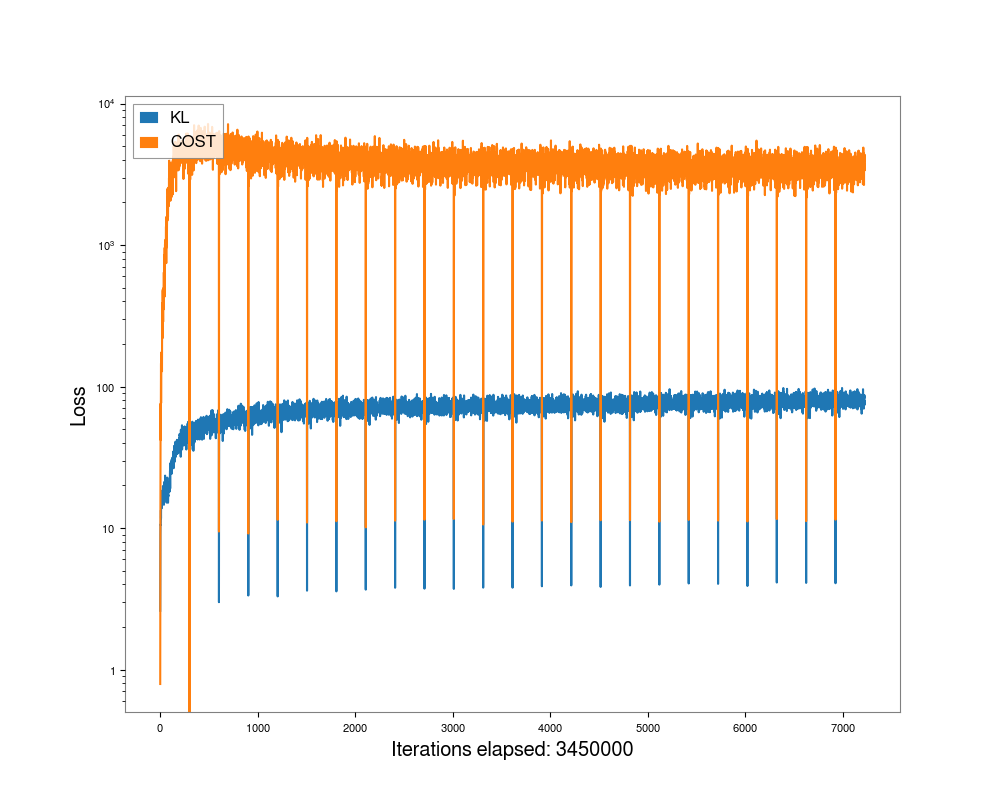
\includegraphics[width=\columnwidth]{images/losses_logscale.png}
    \caption{\label{fig:loss_log} Loss plot with the cost, KL, and total loss
values plotted as a function of the total number of training iterations. We can
conclude that our neural networks have converged to their optimal state when
the slope of our loss curves are close to zero.~\chris{OK, this is the
definition of vague. You don't need to discuss training stopping criteria in
the caption, you siply have to describe what is being plotted. As a general
rule for all captions leave the interpretation of the results to the main
paper. Regarding the plot content, first you need to plot this with x-axis log
scale and y-axis linear scale and also not mess with the signs of the
components. Clearly the comb-like pattern has to be removed somehow - I know
that you'll just do the whole thing again without intermediate plotting. Place
the legend in a more appropriate corner.}} 
\end{figure}

%
% Test procedure
%
After training has completed, we simply feed $\textrm{E}_1$ our test GW signals
$y$. We take the output from $\textrm{E}_1$, and draw latent space samples 
$z_1$. Our
$z_1$ samples are then combined with our test GW signals $y$ and fed
as input to our pre-trained decoder network. The decoder network returns a set
of moments $\mu^{j}_1$ which describe a multivariate Gaussian distribution.
We may then draw random $x$ realisations from that function and is representative of posterior samples from the target
distribution $p(x|y)$. The entire distribution may be represented by 
simply repeating this procedure with the same input data many times over  
(see Eq.~\ref{eq:latent_model}).

%%%%%%%%%%%%%%%%%%%%%%%%%%%%%%%%%%%%%%%%%%%%%%%%%%%%%%%%%%%%%%%%%%%%%%
% RESULTS
%%%%%%%%%%%%%%%%%%%%%%%%%%%%%%%%%%%%%%%%%%%%%%%%%%%%%%%%%%%%%%%%%%%%%%
%
% Intro to the results - what are we trying to do?
%
We present results on $25$ \ac{GW} test waveforms using machine learning 
(\ac{CVAE}s). Posteriors produced by the \texttt{Bilby} inference library~\cite{1811.02042} are used as a benchmark 
in order to asses the efficiency and quality of our machine learning approach 
with the existing most optimal method for posterior sampling. We apply a prior on both component masses which ranges from $35 - 50$
solar masses, a phase prior from $0 - 2\pi$, a distance prior from  $1\textrm{Gpc} - 3\textrm{Gpc}$, and a time of coalesence prior from
from $-0.1$---$0.1$s. All time of coalescence test set
parameters are fixed at $0.5$s
within the $1$s time window~\chris{why do we do this? If we mention it then we
need to motivate it}. The parameters we are not interested in estimating are all fixed (except for phase). we use waveforms that have a duration of 1 second, sampling frequency
of 256Hz, fixed sky position (right ascension ($\alpha$), declination ($\delta$)), inclination angle ($\theta_j$), polarization angle ($\psi$) and a spin of zero. We allow 5 parameters to vary: component masses $m_1$ and $m_2$, luminosity
distance, time of coalescence and phase, where phase is marginalized
out. It should be noted that nuisance parameters can (if desired) be 
marginalized out in the machine learning training procedure itself, rather 
than after training. \texttt{Bilby} on the other hand must explore the initial 
phase space when performing full inference. The waveform
model ($h$) used is
\texttt{IMRPhenomPv2}~\cite{1809.10113} with a minimum cutoff frequency of
20Hz. \ac{CVAE} posterior results are produced by passing our $25$ \ac{GW} 
waveforms as input to a pre-trained \ac{CVAE} decoder and sampling until we have 
generated $\sim5000$ posterior samples per parameter, per \ac{GW} signal 
\texttt{Bilby} is passed the same $25$ \ac{GW} test waveforms and we randomly sample $\sim5000$ samples from \texttt{Bilby} posteriors to be used as our benchmark.


%
% discuss codebase which we use to generate waveforms, sampling frequency, and
% parameter space
%

%
% K-L divergence results
%
\begin{figure}
    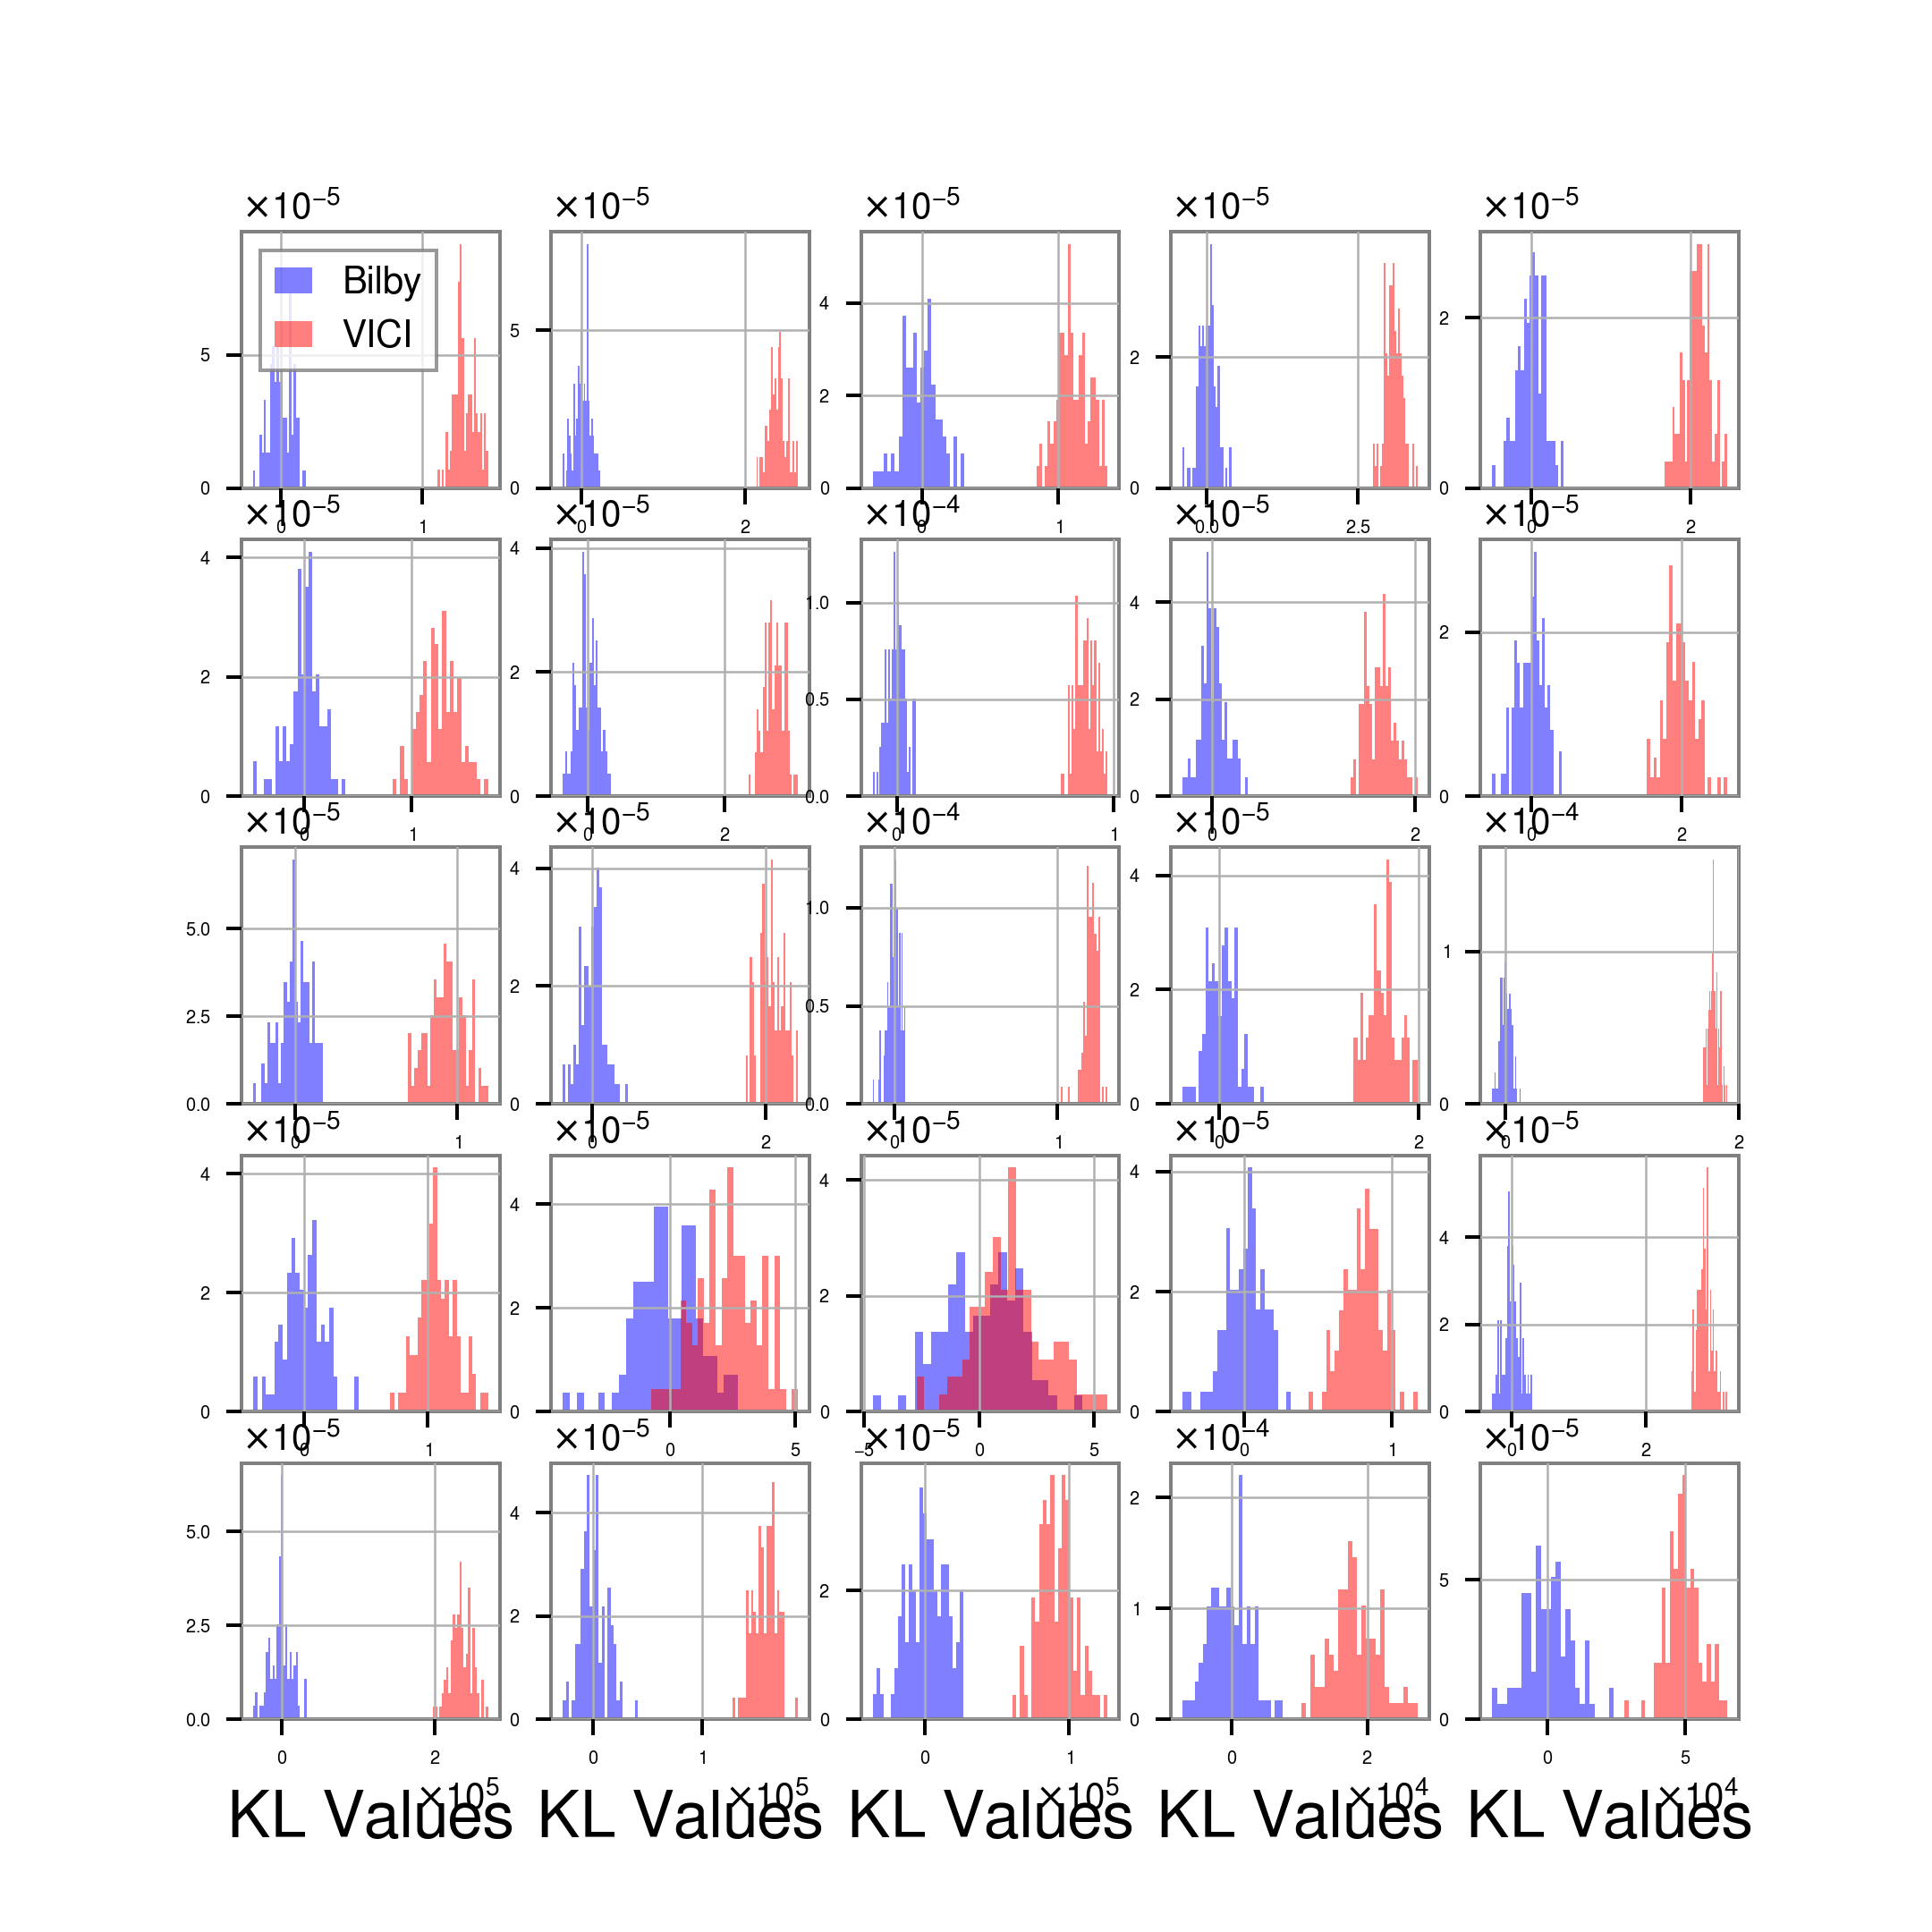
\includegraphics[width=\columnwidth]{images/hist-kl_0.png}
    \caption{\label{fig:kl_results} Histograms of 25 different test GW signal
\ac{KL} divergence values.  Red denotes predictions from the CVAE and blue denotes
predictions from \texttt{Bilby}.~\chris{OK, practical plotting comments first.
We can't have 5x5 results shown here. You need to fix the font sizes and
probably use a log scale on the y-axis. The bins sizes are too small in most
histograms (try to use 100 bins across the complete range in each plot). Only
use one central x-axis label (not one for every plot). Also add a central
y-axis label stating $p(\text{KL})$. For the caption you need to provide more
details of what is being shown. You don't get multiple KL values for a given
pair of posteriors so how did you generate this? Now, in general - what to do
about showing the KL values? Here's what I suggest. I think we need to do $N$
test sets where $N>25$ but 25 will suffice for now. For each of these cases you
need to run Bilby with all the different samplers and each sampler run twice.
Then you can make a single plot showing the histogram (made from $N$
realisations) of KL values. You would have a histogram from each sampler vs
every other sampler (so 3 samplers plus VItamin makes 4 which results in 10
histograms). When  you do one sampler against itself you use the 2nd run. There
would be no bootstrapping. What do you think?}}
\end{figure}
%
In Fig. \ref{fig:kl_results} we show histograms of \ac{KL} divergence values on $25$
test GW samples. The \ac{KL} divergence is computed $100$ times per test sample
through the initialization of random splits. We compute the KL divergence on
\ac{CVAE} results (red) by comparing \ac{CVAE} predictions to \texttt{Bilby}
predictions. Our benchmark \texttt{Bilby} (blue) results are computed by
choosing random $50/50$ splits between results from the same \texttt{Bilby}
produced posterior.~\chris{I think this text will need to change based on
changing the KL plot (see caption comments). In general though, looking at the
results themselves it's clear that we're not too far away from overlapping
distributions in most cases. I guess it depends on how much we push. Is there
any correlation between the 2 obviously overlapping test cases and their signal
properties?}

%
% AD results
%
\begin{figure}
    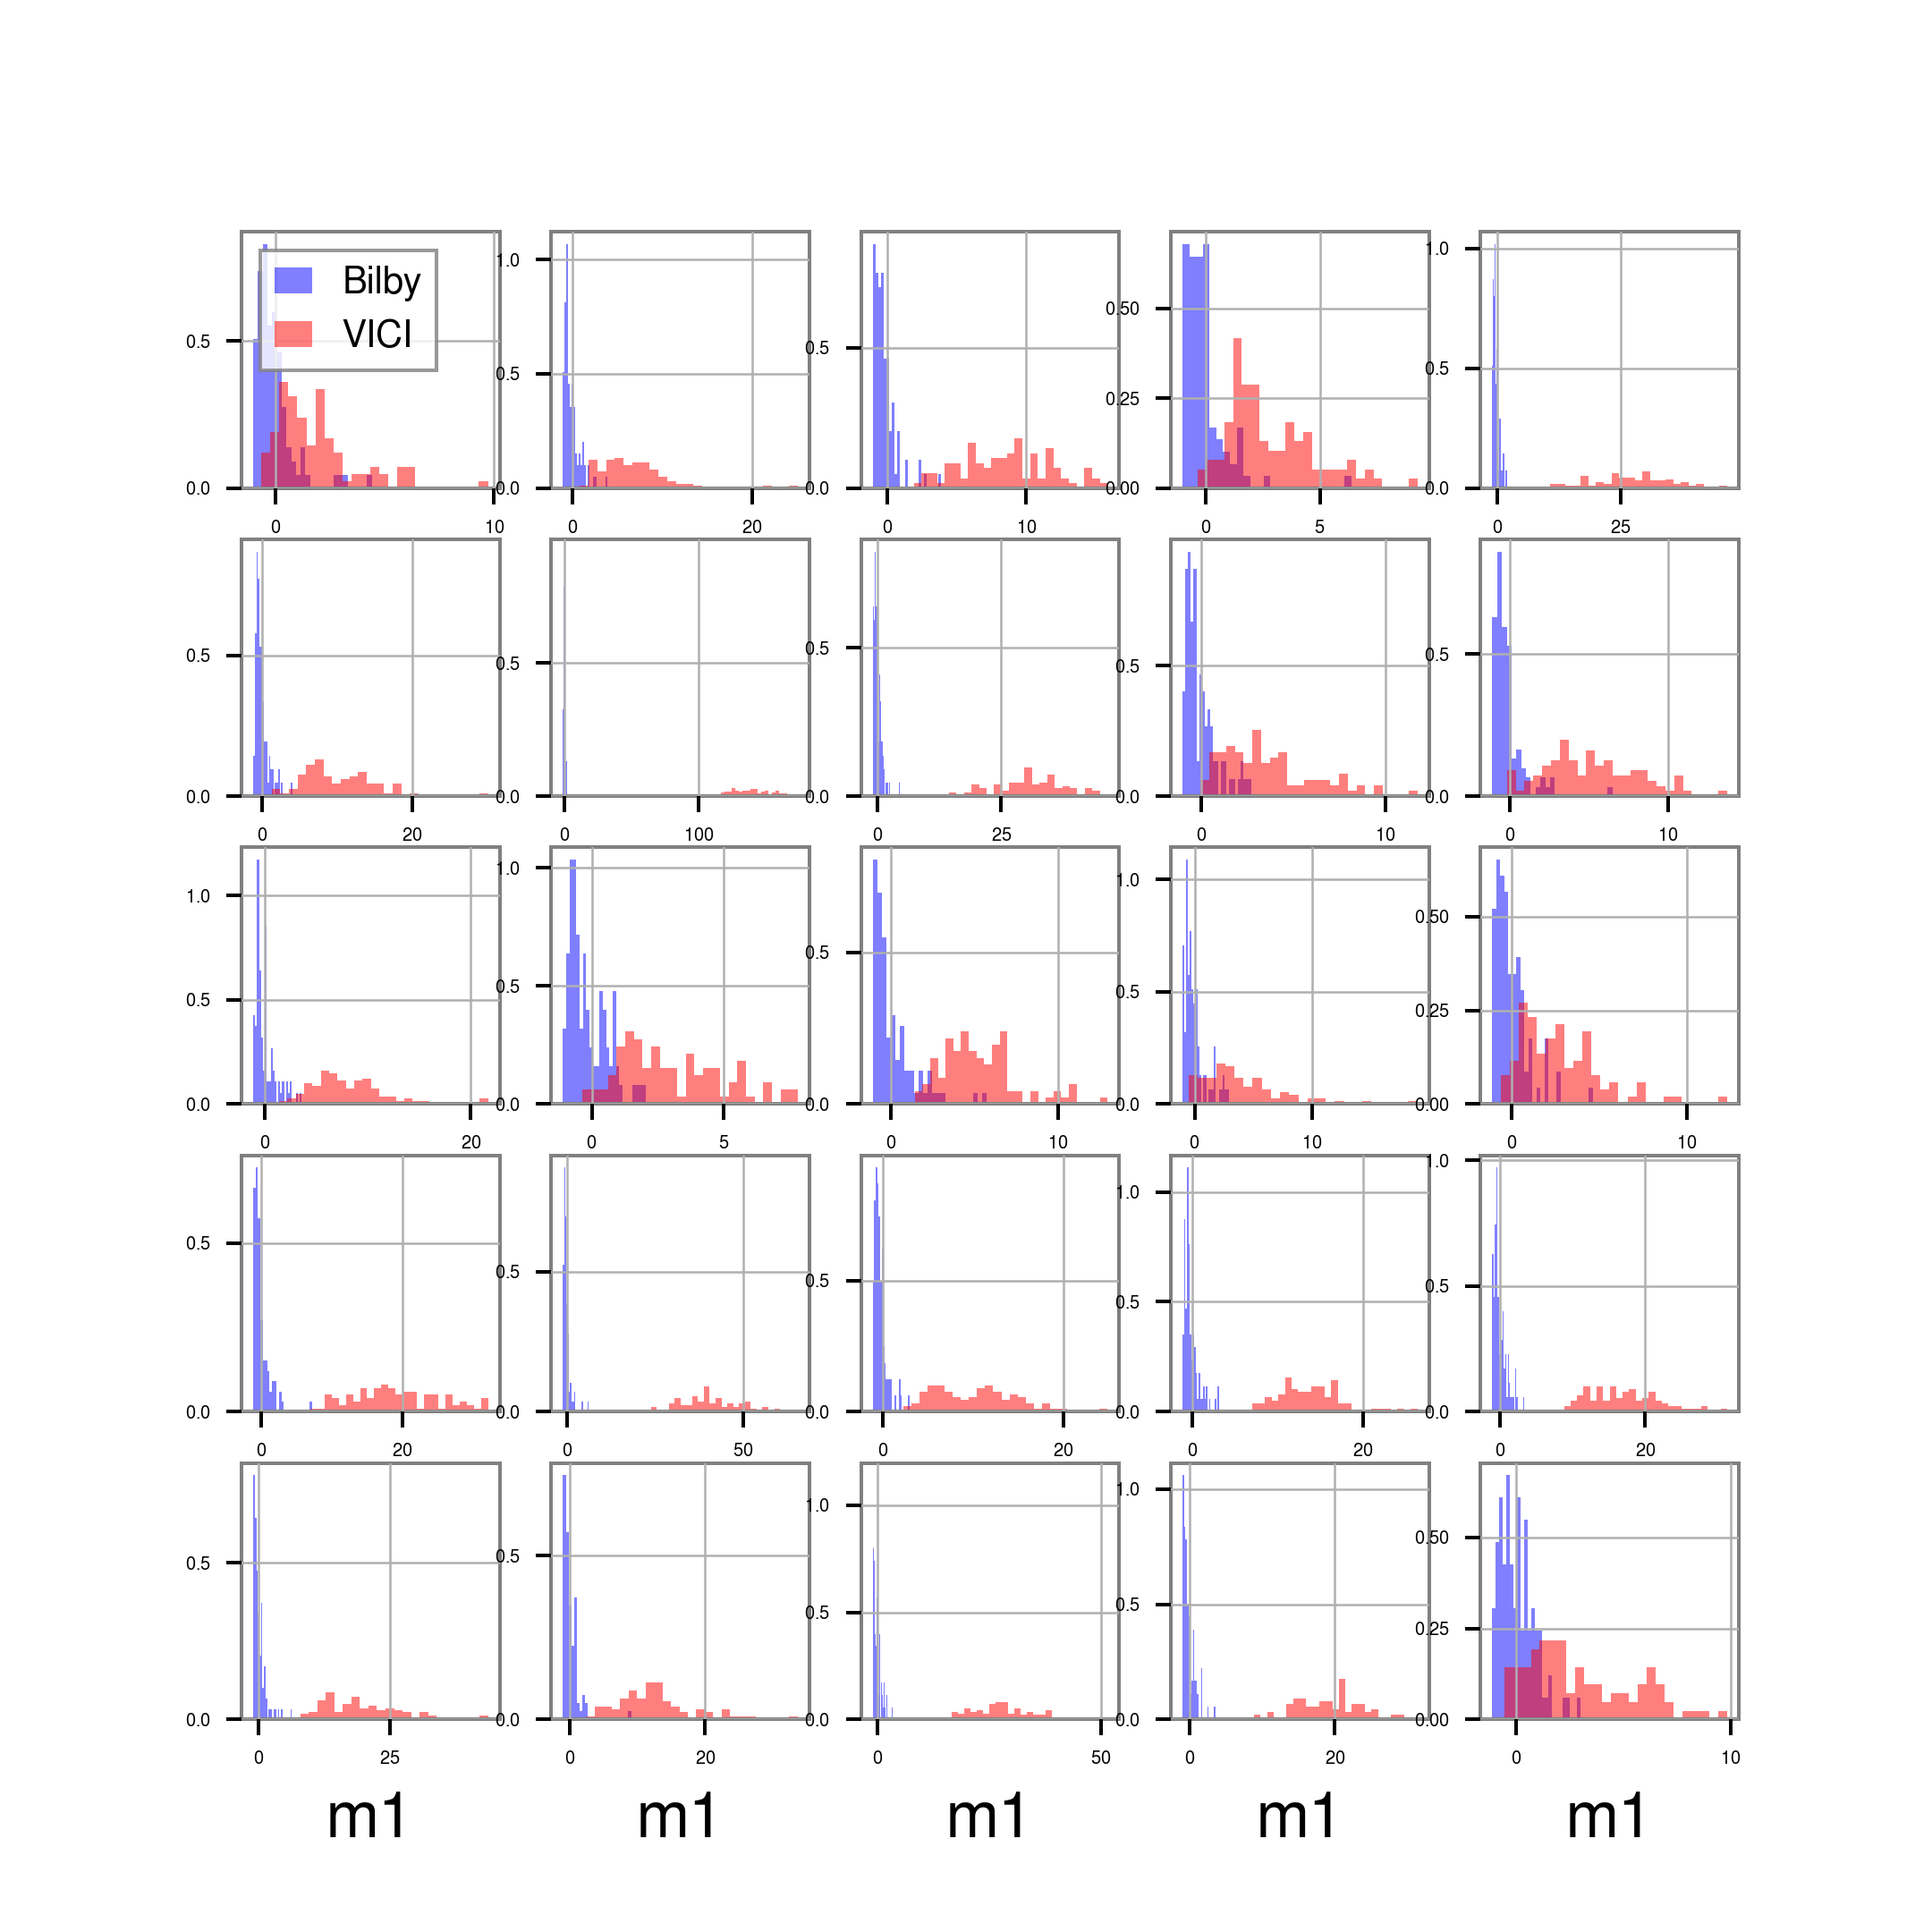
\includegraphics[width=\columnwidth]{images/hist-ad_0.png}
    \caption{\label{fig:ad_results} Histograms of 25 different test GW signal
Anderson-Darling (AD) statistic component mass 1 values. Distributions which
are similar will have AD values which are close to 0.  Red denotes predictions
from the \ac{CVAE} and blue denotes predictions from
\texttt{Bilby}.~\chris{Please see the suggested changes in
Fig.~\ref{fig:kl_results} and apply the same here. Results wise this doesn't
look too bad and a bit more tuning might get everything to overlap in a nicer
looking way. Also, the x-axis label is wrong.}}
\end{figure}
%
In Fig.~\ref{fig:ad_results} we show histograms of \ac{AD} statistic results
computed over $100$ iterations per test sample.  The \ac{AD} statistic is a
1-dimensional figure of merit, so Fig.~\ref{fig:ad_results} only illustrate
results from predictions on $m_1$.~\chris{but why only $m_{1}$? If there is a
reson then state it.} The closer \ac{AD} statistic values are to zero, the more
likely that the two distributions being compared are drawn from the same
distribution~\chris{2 distributions can't be drawn from the same distribution.
Check your language.}. As can be seen in Fig.~\ref{fig:ad_results} there is
some overlap between the machine learning predictions and our benchmark
\texttt{Bilby} results.~\chris{hopefully if/when we improve the results the AD,
KL, and KS statsistics will all be reasonably overlapping and we can say a bit
more about it.}

%
% P-P plot
%
\begin{figure}
    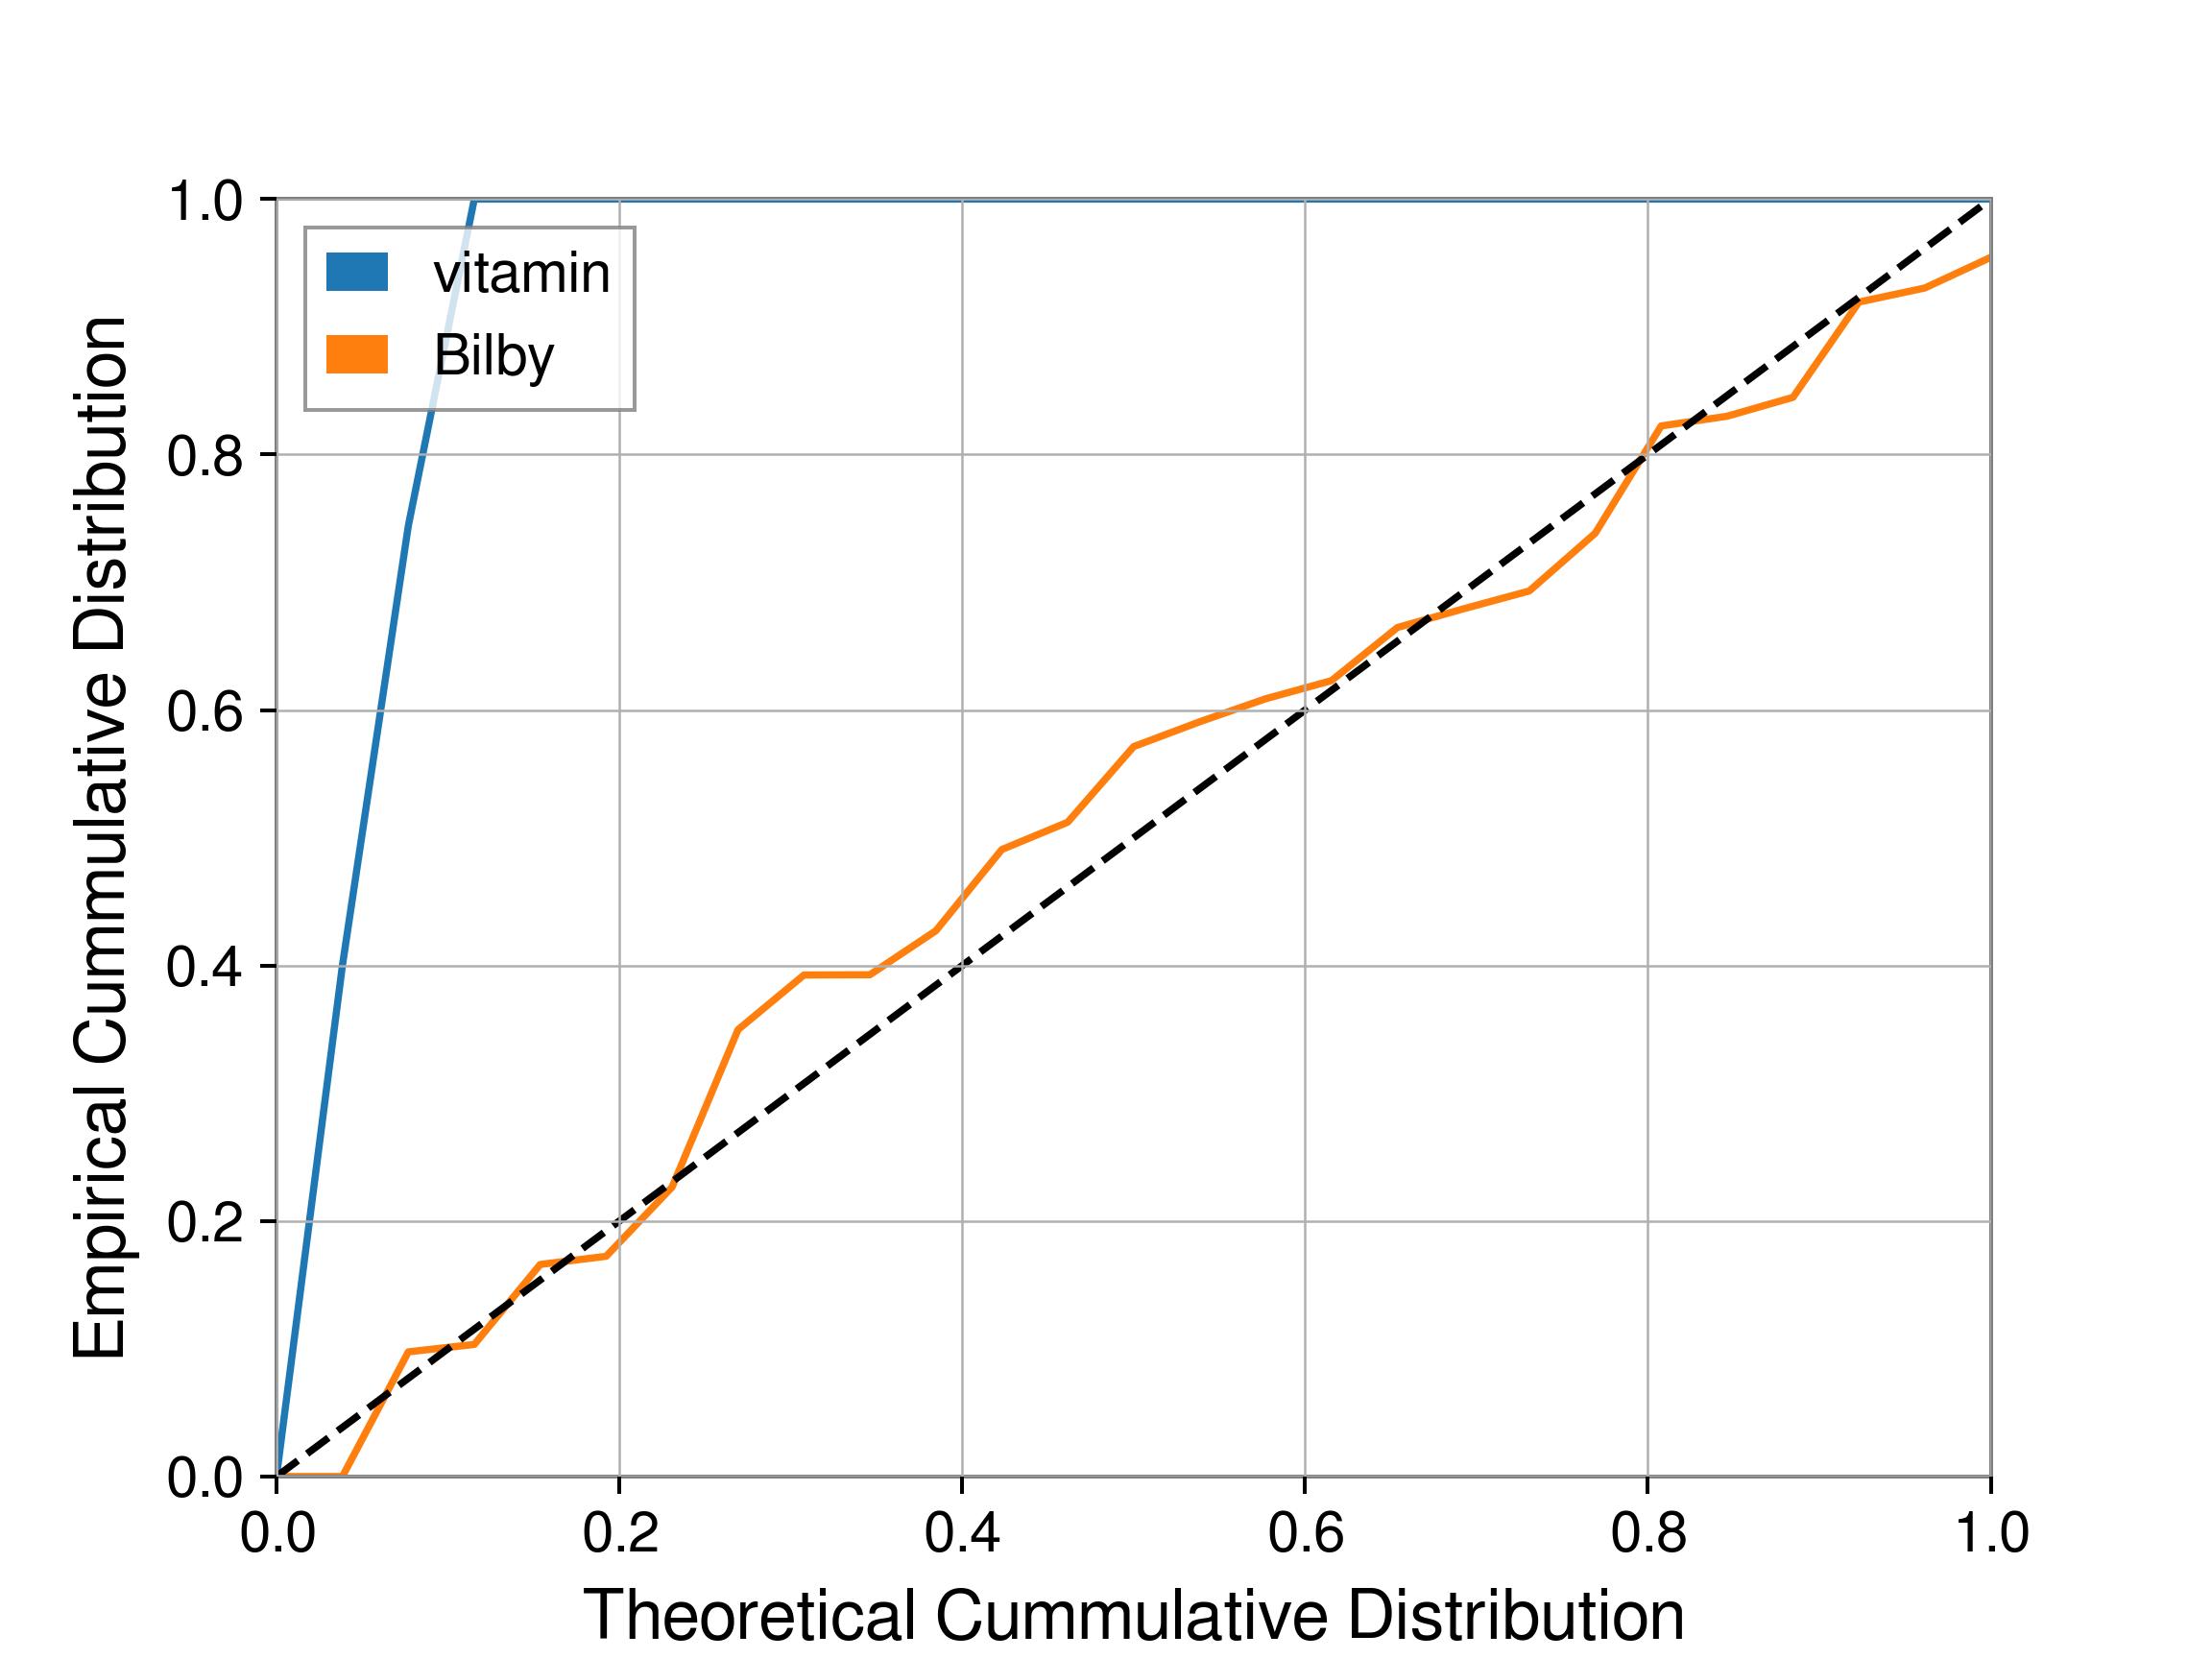
\includegraphics[width=\columnwidth]{images/latest_pp_plot.png}
    \caption{\label{fig:pp_plot} P-P plot using $100$ unique test samples and
$5000$ posterior sample predictions per test sample.  The x-axis denotes the
theoretical cummulative distribution whereas the y-axis denotes the predicted
cummulative distribution.~\chris{we might have to work on the description of
the axes - maybe use the same notation that has been used in the GW PE papers
that include p-p plots. Obviously this plot is quite worrying but I can't see
why you get these results looking at the test data posterior comparison. Can
you please check the p-p plot code - you should run it on the Bilby samples as
a reference anyway. To make the plot more interesting you could also plot
curves from each of the different bilby samplers (since you'll have to run
those anyway). Also, try to make the plot square - there is supposed to be a
symmetry between the axes.}} 
\end{figure}
%
In order to show that our results are consistent with the truth, we have
additionally plotted probability-probability (p-p) plots in
Fig.~\ref{fig:pp_plot}. On the y axis is plotted the predicted cummulative
distribution and on the x axis is plotted the theorectical distribution.
Perfect alignment with the truth~\chris{No, a diagonal p-p plot is only
possible with infinite data but consistent with diagonal is indicative that the
Bayesian probability distributions are consistent with the frequentist
interpretation - that the truth will lie inside the $X\%$ probability contour
with a frequency of $X\%$ of the time.} is illustrated by the black dashed
diagonal line, while our empirical alignment is shown in the blue
line.~\chris{as mentioned in the figure caption comments, please add p-p plot
curves for the other samplers run on the same test data.} 

%
% 1-D overlap results
%
\begin{figure}
    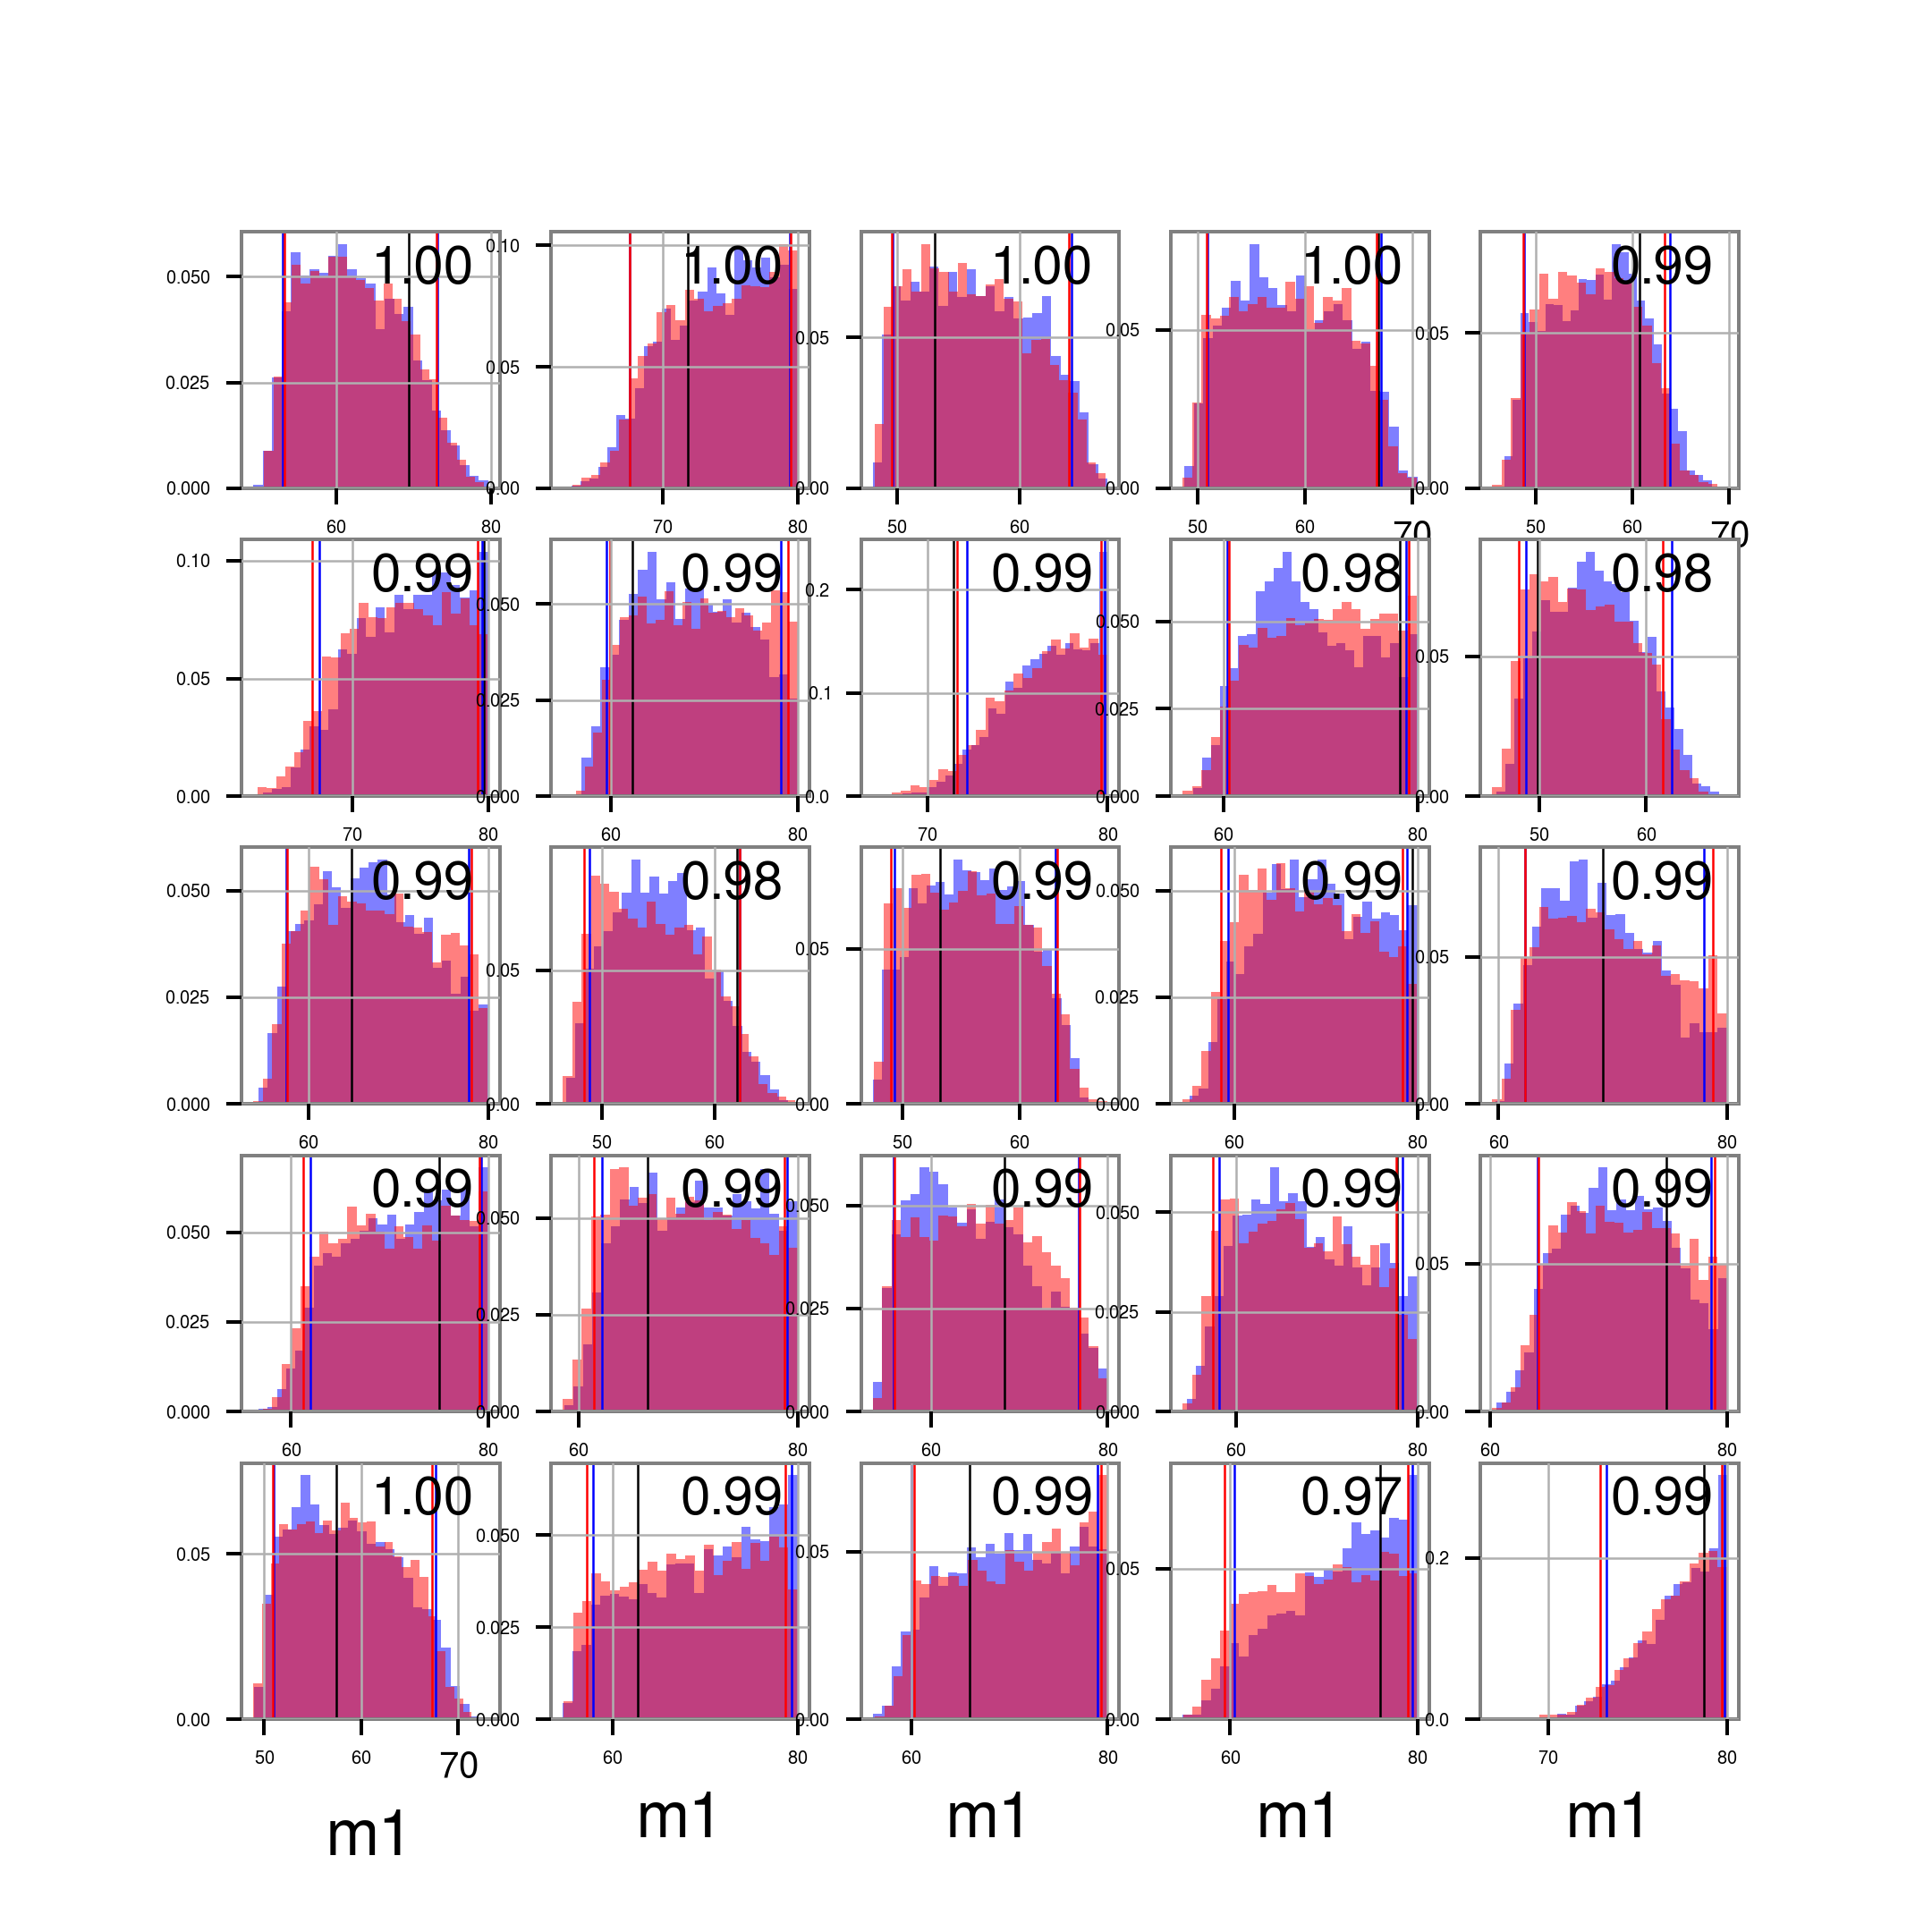
\includegraphics[width=\columnwidth]{images/latest-1d_0.png}
    \caption{\label{fig:1D_overlap} Histograms of 25 different test GW signal
component mass 1 values.  Numbers in the upper right-hand corner denote overlap
values where 1 means $\sim{100}\%$ overlap and 0 means $\sim{0}\%$
overlap.~\chris{we shouldn't use overlaps unless we define how they're
calculated in the text. I think that overlaps are not something we need at this
point. Don't remove them yet since they are still useful to us but they should
be removed from the final plots.} Red denotes predictions from CVAE predictions
and blue denotes predictions from \texttt{Bilby}.~\chris{the 1 and 2D posterior
plots should be represented as a corner plot for a single test data realisation
- this plot should span 2 columns - it is our primary plot. Also the way in
which the bilby and VItamin samples are overlayed needs to be changed. Now that
the overlap is so good we need to be able to see how good it really is. Can I
ask that the bilby results be represented as contours (68,90,95\%) and the
VItamin results be shown as samples OR also as contours. If both are contours
then the VItamin contours should be filled and the bilby contours should just
be lines (VItamin in blue and bilby in red I think). Whatever colours are used
then they should be consistent throughout the paper.}}
\end{figure}
%
% 2D scatter plot
%
\begin{figure}
    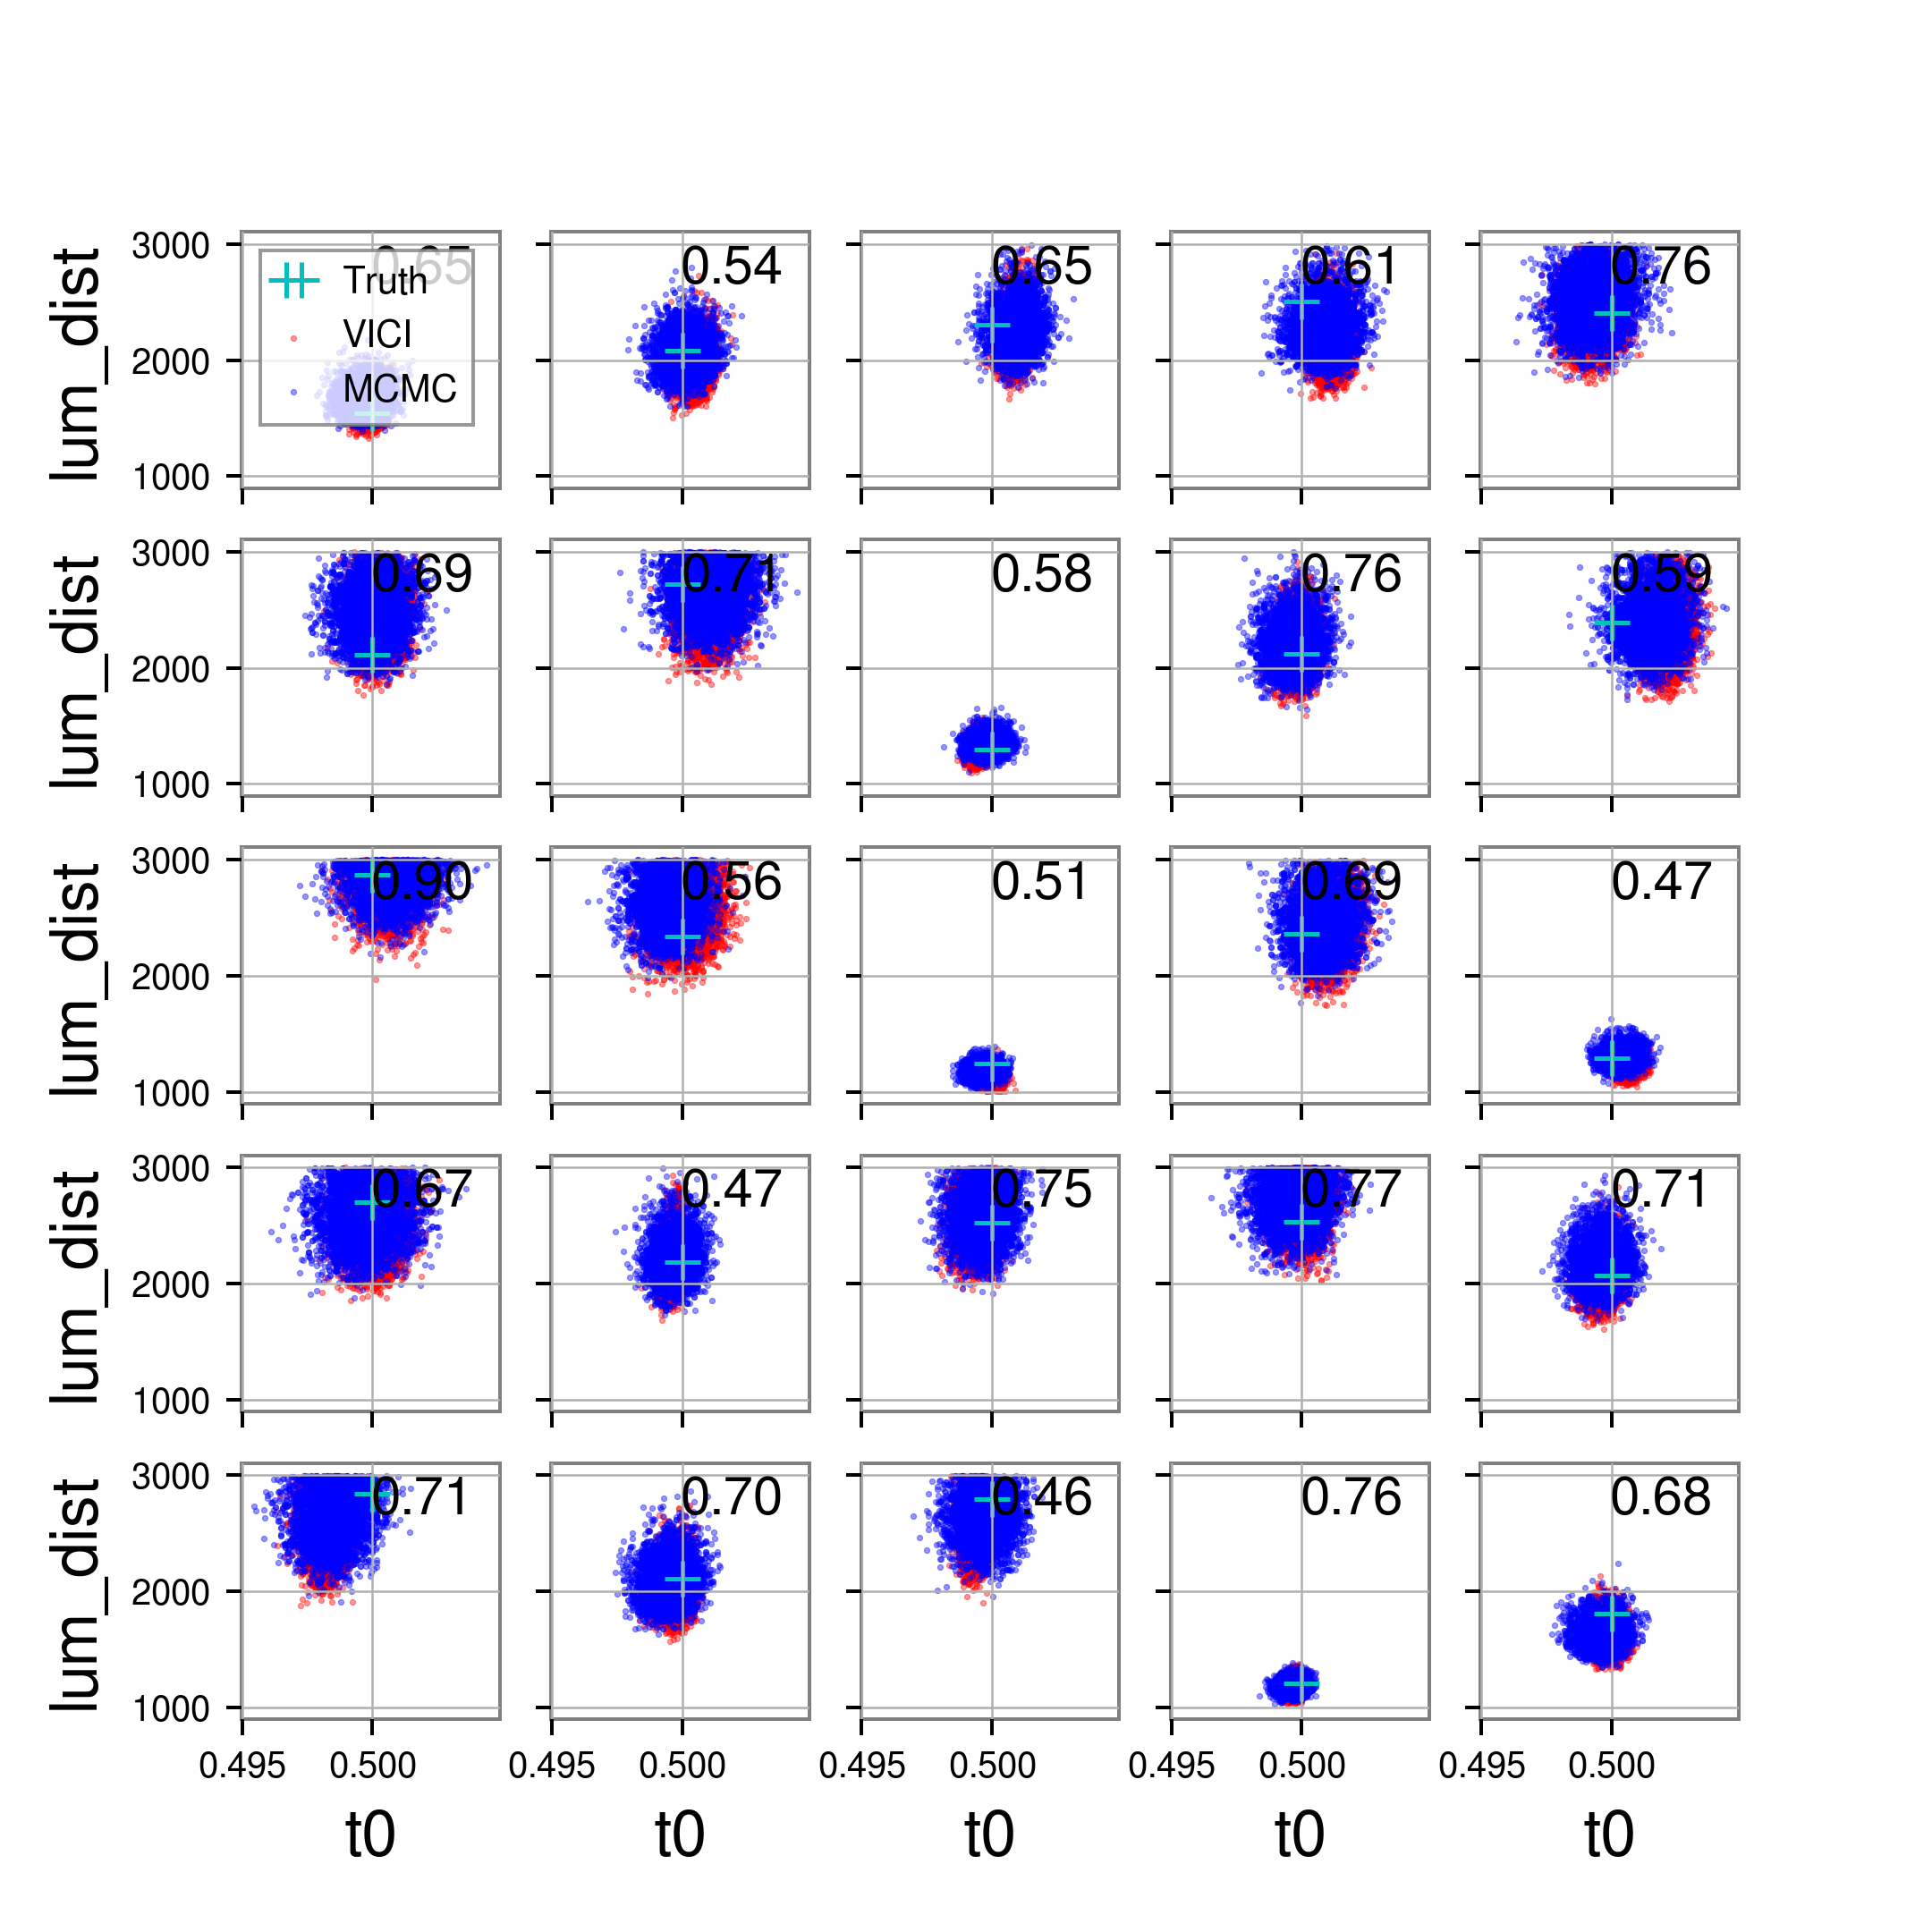
\includegraphics[width=\columnwidth]{images/posteriors_13.png}
\caption{\label{fig:lum_dist-t0_scatter} This figure illustrates 25 different
test GW samples with $5000$ posterior samples from both \texttt{Bilby} and our
CVAE plotted. Red denotes predictions from the CVAE and blue denotes
predictions from \texttt{Bilby}. Luminosity distance is plotted as a function
of time of coalescence with 4-dimensional overlap values printed in the upper
right-hand portion of each subplot.\chris{see Fig.~\ref{fig:1D_overlap} caption
for comments}}
\end{figure}
%
We can further illustrate the accuracy of our machine learning predictions by
directly plotting the samples generated by our CVAE and \texttt{Bilby}
superimposed on each other.  In Fig. \ref{fig:1D_overlap}, we histogram
predictions sampled from the posterior through both \texttt{Bilby} (blue) and
our CVAE (red).  As can be clearly seen, the overlap between both
\texttt{Bilby} and the CVAE is extremely high in the $m_1$ parameter space.
Additional proof of high overlap between posteriors can also be seen in Fig.
\ref{fig:lum_dist-t0_scatter} where we plot samples from both \texttt{Bilby}
(blue) and the CVAE (red) posteriors with luminsoity distance as a function of
$t_0$. 

\chris{One more thing to add, especially if the other KL, AD, and PP plots
aren't convincing, is a plot displaying 1D confidence bounds compared between
bilby and VItamin. Imagine a plot with the x-axis as distance and the y-axis
steps through test data with increasing true distance. for each test data you
plot 2 error bars horizontally (one for bilby and one for VItamin) spanning the
range of 90\% confidence. You would hopefully get nearly identical pairs of
errorbars stacked vertically. Technically you could do this for all parameters
(and you should) but we might only put one of the plots in the paper (if at
all).}

\chris{Also, what about the speed argument? We need to have a final number for
how long it takes to train our network including the time it takes to generate
the data. We then need (easy to get) numbers for how fast it takes to generate
samples from the trained network - this is crucial and we need to see if the
post-generation pruning of the parameter space slows us down. All of this needs
to be compared fairly apples-to-apples with the bilby runs on the same data. We
have to be very careful in equating our speed to that of real runs at full
timing resolution because we will be criticised for being unfair. If we have
time (which is unlikely) then it would be good to be able to answer questions
like, how does the training and sample generation speed scale with length of
data or network complexity.}

%%%%%%%%%%%%%%%%%%%%%%%%%%%%%%%%%%%%%%%%%%%%%%%%%%%%%%%%%%%%%%%%%%%%%%
% CONCLUSIONS
%%%%%%%%%%%%%%%%%%%%%%%%%%%%%%%%%%%%%%%%%%%%%%%%%%%%%%%%%%%%%%%%%%%%%%
%
% recap and main result
%
\chris{We may be limited in words at this point but it might be good to
reiterate (briefly) the challenges faced in PE for the GW field. Then go on to
say what we've shown.} In this letter we have demonstrated that we are able to
reproduce, to a high degree of accuracy~\chris{we will be careful with this
phrasing}, posteriors \chris{probability distributions} generated from Bayesian
inference using machine learning. This is accomplished through the use of
variational autoencoders trained on over 1 million~\chris{the numbers are
irrelvent at this stage - especially if you're not going to mention all of the
other equally important ones.} whitened~\chris{whitening is not important - all
approaches use whitening, it is a technicallity to only be mentioned in
passing.} simulated \ac{GW} signals. By building a neural network model which,
when trained, can reproduce the true posterior in less than a second~\chris{we
will verify and firm-up this number - especially since its problem dependent.},
we have demonstrated that neural networks can achieve the same
sensitivity~\chris{there isn't really any sensitivity here - it's not a search.
It's more like quality of results or optimality.} as that of \chris{the trusted
benchmark of} Bayesian inference.

%
% discuss the near term CBC implications and why this is a game-changer
%
The significance of achieving similar sensitivities~\chris{not sensitivities}
to Bayesian inference is most evident in the orders of magnitude speed-up in
performance~\chris{more like orders of magnitude gains in speed - the
performance is idemtical (hopefully).}. The increase in speed will help the
LIGO-Virgo-Kagra calibration alert our electromagnetic follow-up partners with
minimum latency.~\chris{you need to expand upon this a bit more - mention
GW170817, catching prompt EM emission with super-fast PE estimates, this will
highlight the fact that we haven't shown the sky inference. The estimated
future detections for BNS (give numbers) will currently swamp our computer
resources. Whilst BBH are relatvely easy we will also be swamped with far more
of these. Our approach will provide (potentially) full-PE on BBH signals in
seconds on a single GPU. Also the trained pipeline is incredibly portable - 1
saved network and a small script to feed in new data - anyone can get results.
Also talk about priors and how although the analysis assumes priors, we can
train boxes to essentially produce samples from the likelihood - people can
then resample from them according to their own prior choices.} 

\chris{I had another thought. This is also very important for population
studies since populations can be generated and now analysed in full-Bayes many
times very quickly.}

%
% future work, current limitations and prospects
%
\chris{You need to be upfront about the corners that we've cut and the work
that needs to be done. Why are we doing a low sample rate? Why are we limiting
the mass space? Why did we only do 1 detector? Is there any reason we can't do
all of those things in the near future? What about the things that we want to
do that are extra to the normal - like dealing with non-Gaussian noise (we
could train on real detector data) - we wouldn't be affected by the type of
glitch that delayed the confirmed detection and analysis of GW170817- our
results wouldn't technically depend on our choices of whitening whereas current
methods do. } Our work can further be expanded upon by including a variety of
other \ac{GW} sources such as Neutron star - black hole (NSBH)~\chris{no need
for an acronym if it's only ever used once.} and \ac{BNS} mergers at higher
sampling frequencies. We have yet to demonstrate the effectivness of our method
on additional parameters such as sky location and inclination angle, the
benefits of which would be best realized in an end-to-end inference pipeline.
Such a pipeline would be of great importance as the detectors increase up to
their full potential design sensitivities.~\chris{nice but think bigger - this
or something like it will form the basis of PE for the next 20 years.}

\chris{Whether there is another paragraph or not, end on a postive note.}

%%%%%%%%%%%%%%%%%%%%%%%%%%%%%%%%%%%%%%%%%%%%%%%%%%%%%%%%%%%%%%%%%%%%%%
% METHODS
%%%%%%%%%%%%%%%%%%%%%%%%%%%%%%%%%%%%%%%%%%%%%%%%%%%%%%%%%%%%%%%%%%%%%%
\section{Methods}
%
Put methods in here.  If you are going to subsection it, use
\verb|\subsection| commands.  Methods section should be less than
800 words and if it is less than 200 words, it can be incorporated
into the main text.

\subsection{Whitening} \label{whiten_sec}

In order to ensure 
that there is equal power accross all
frequency bins of our signal, we ensure that the noise is whitened Gaussian
noise. We whiten using a single detector (H1) power spectrum density derived from the
Advanced LIGO design sensitivity curves \cite{2016LRR....19....1A}. 

\subsection{Nested Sampling} \label{nested_sec}
%
% Describe nested sampling algorithm
%
If we would like to find the results for a particular parameter, 
we simply marginalize over all unwanted parameters 

\begin{equation}
    p(x_1|y) = \int dx_2 ... dx_N p(x|y).
\end{equation}

There are several algorithms which may be used to sample from the posterior
distribution of astrophysical GW source parameters \cite{PhysRevD.64.022001,
skilling2006,10.1111/j.1365-2966.2011.20288.x}. The
algorithm which is used in our case is the nested sampling algorithm. Nested
sampling takes a multi-dimensional evidence integral calculation (fully
marginalized likelihood) and transforms it into a more manageable 1-D integral
, where evidence is the integral of the likelihood 
multiplied by the prior over all parameters of the model $h$ ~\cite{1409.7215}

\begin{equation}
    Z = p(y|h) = \int dx_1 ... dx_n p(y|x,h)p(x|h).\label{eq:evidence}
\end{equation}

%
% More nested sampling description
%
The first step of the nested sampling algorithm starts by generating an initial
set of live points made from the prior distribution. The likelihood for each
point is calculated and the point with the lowest likelihood is removed. The
removed sample is then replaced with a new sample which has a higher
likelihood. This cycle repeats itself until a predefined stopping threshold is
achieved \cite{1409.7215} . Samples from the posterior may be drawn by randomly
selecting from both all current 'live' points and all previously removed 'live'
points.

The nested sampling algorithm is run using
1000 live points and has a predefined stopping criteria of $0.1$~\chris{expand
upon what the stopping criteria means. This is related to the evidence
calculation and the tolerance on that result}. The sampler takes $\mathcal{O}(3
\: \textrm{minutes})$ to converge~\chris{jargon. What does converge mean to the
average Nature reader?}. After the nested sampler has converged~\chris{jargon}, we draw
samples~\chris{too technical with not enough explanation. The \texttt{Bilby} analysis
produces posterior parameter estimates and does so by supplying the user with
samples drawn from that distribution.} and produce a posterior on the
astrophysical \ac{GW} source parameters we are trying to estimate.

\subsection{Loss function derivation} \label{lossDer_sec}

This section is to be rephrased into appropriate language but for now I will
add my interpretation of the loss function and the design of the network.

We begin with the statement defining the aim of the analysis. We wish to obtain
a function that reproduces the posterior distribution (the probability of our
physical parameters given some measured data). We define the cross entropy
between 2 distributions as
%
\begin{equation}\label{eq:cross_ent}
H(p,r) = -\int dx\, p(x|y) \log r_{\theta}(x|y)
\end{equation}
%
where we have made the distributions explicitly conditional on $y$ (our
measurement). In this case $p(x|y)$ is the target distribution (the true
posterior) and $r_{\theta}(x|y)$ is the parametric distribution that we will
use neural networks to construct. In this case $\theta$ represents the
trainable neural network parameters. 

The cross-entropy is minimised when $p(x|y)=r_{\theta}(x|y)$ and so by maximising
%
\begin{equation}\label{eq:cost1}
C = \text{E}_{p(y)}\left[\int dx\,p(x|y) \log r_{\theta}(x|y)\right]
\end{equation}
% 
where $\text{E}_{p(y)}[\dot]$ indicates the expectation value over the
distribution of measurements, we therefore make the parameteric distribution as
similar to the target for all possible measurements $y$.

Converting the expectation value into an integral over $y$ weighted by $p(y)$
and applying Bayes theorem we obtain
%
\begin{equation}\label{eq:cost1}
C = \int dx\,p(x)\int dy\,p(y|x)\log r_{\theta}(x|y)
\end{equation}
%
where $p(x)$ is the prior distribution on the physical parameters $x$.

The conditional variational autoencoder network outlined in
Fig.~\ref{fig:network_config} makes use of a conditional latent variable model.
Our parameteric model is constructed from the product of 2 seperate
distributions marginalised over the latent space
%
\begin{equation}\label{eq:latent_model}
r_{\theta}(x|y) = \int dz\,r_{\theta_{1}}(z|y)r_{\theta_{2}}(x|z,y).
\end{equation}
%  
We have used $\theta_{1}$ and $\theta_{2}$ to indidate that the 2 seperate
networks modelling these distributions will be trained on these parameter sets
respectively. Both new conditional distributions are modelled as $n_{z}$
dimensional multivariate uncorrelated Gaussian distributions (governed by their
means and variances). However, this still allows $r_{\theta}(x|y)$ to take a
general form (although it does limit it to be unimodal).  

One could be forgiven in thinking that by setting up networks that simply aim
to maximise $C$ over the $\theta_{1}$ and $\theta_{2}$ would be enough to solve
this problem. However, as shown in~\cite{NIPS2015_5775} this is an intractable
problem and a network cannot be trained directly to do this. Instead we define
a recognition function $q_{\phi}(z|x,y)$ that will be used to derive an
\ac{ELBO}.

Let us first define the Kullback–Leibler divergence between 2 of our
distributions as
%
\begin{equation}\label{eq:kl}
\text{KL}\left[q_{\phi}(z|x,y)||r_{\theta_{2}}(z|x,y)\right] = \int dz\,
\log\left(\frac{q_{\phi}(z|x,y)}{r_{\theta_{2}}(z|x,y)}\right).
\end{equation}
%  
It can be shown that after some manipulation that
%
\begin{equation}\label{eq:elbo1}
\log r_{\theta}(x|y) = L + \text{KL}\left[q_{\phi}(z|x,y)||r_{\theta_{?}}(z|x,y)\right]
\end{equation}
%
where the \ac{ELBO} $L$ is given by
%
\begin{equation}\label{eq:elbo2}
L = \int dz\,
q_{\phi}(z|x,y)\log\left(\frac{r_{\theta_{2}}(x|z,y)r_{\theta_{1}}(z|y)}{q_{\phi}(z|x,y)}\right)
\end{equation}
%
and is so-named since $\text{KL}$ cannot be negative and has a minimum of zero.
Therefore, if we were to find a $q_{\phi}(z|x,y)$ function (optimised on
$\phi$) that minimised the KL-divergence then we can state that
%
\begin{equation}
\log r_{\theta}(x|y) \geq L.
\end{equation}
%
After some further manipulation of Eq.\ref{eq:elbo2} we find that
%
\begin{align}\label{eq:logr}
\log r_{\theta}(x|y) \geq & \text{E}_{q_{\phi}(z|x,y)}\left[\log
r_{\theta_{2}}(x|z,y)\right] \nonumber\\
&-\text{KL}\left[q_{\phi}(z|x,y)||r_{\theta_{1}}(z|y)\right].
\end{align}
%
We can now substitute this inequality into Eq.~\ref{eq:cost1} (our cost
function) to obtain
%
\begin{align}\label{eq:cost2}
C \geq & \int dx\, p(x)\int dy\,p(y|x)
\left[\text{E}_{q_{\phi}(z|x,y)}\left[\log r_{\theta_{2}}(x|z,y)\right]
\right.\nonumber\\
&-\left.\text{KL}\left[q_{\phi}(z|x,y)||r_{\theta_{1}}(z|y)\right]\right]  
\end{align}
%
which can in practice be approximated as a stochastic integral over draws of
$x$ from the prior, $y$ from the likelihood function $p(y|x)$, and from the
recognition function, giving us
%
\begin{align}\label{eq:cost3}
C \geq & \frac{1}{N}\sum_{n=1}^{N}\left[\log
r_{\theta_{2}}(x_{n}|z_{n},y_{n})\right.\nonumber\\
&\left.-\text{KL}\left[q_{\phi}(z|x_{n},y_{n})||r_{\theta_{1}}(z|y_{n})\right]\right].
\end{align}
% 
In this case we draw $N$ sets of physical parameter, corresponding data
sets, and draws from the recognition function. It is important to note that
whilst it is true that the KL-divergence between the $q_{\phi}(z|x,y)$ and
$r_{\theta_{2}}(z|x,y)$ (seen in Eq.~\ref{eq:elbo1}) should be minimised and in
an ideal case be equal to zero, that is not the case for the KL-divergence in
Eq.~\ref{eq:cost3}. In this case our aim is to maximise $C$ which implies that
the KL-divergence should be low but not necessarily zero.

We have now set up a system composed of 3 functions that have well defined
inputs and outputs where the mapping of those inputs to outputs is governed by
the parameter sets $\theta_{1},\theta_{2},\phi$. These parameters are the
weights and biases of 3 neural networks acting as (variational) encoder,
decoder, and encoder respectively. To train such a network one must connect the
inputs and outputs appropriately to compute $C$ and back-propogate cost
function derivatives to update the network parameters. The network structure
shown in Fig.~\ref{fig:network_config} shows how for a batch of $N$ sets of $x$
and corresponding $y$ values first both $x$ and $y$ are fed into the encoder 2
network that produces the means and variances of the latent space $z$
describing the $q_{\phi}(z|x,y)$ distribution function. Next (the order does
not matter) the data $y$ alone is passed into the encoder 1 network that
produces the means and variances of the latent space $z$ describing the
$r_{\theta_{1}}(z|y)$ distribution function. Given the parameters of these
Gaussian (diagonal covariance matrix) distributions the $\text{KL}$-divergence
is computed as
%
\begin{align}\label{eq:klgauss}
\text{KL}\left[q_{\phi}(z|x_{n},y_{n})||r_{\theta_{1}}(z|y_{n})\right] =&
\frac{1}{2}\sum_{j=1}^{n_{z}}\left[\frac{\sigma_{q,j}^{2}}{\sigma_{r,j}^{2}} +
\frac{(\mu_{r,j}-\mu_{q,j})^{2}}{\sigma_{r,j}^{2}}\right.\nonumber\\ 
&\left.+
\log\left(\frac{\sigma_{r,j}^{2}}{\sigma_{q,j}^{2}}\right)\right] -
\frac{n_{z}}{2}
\end{align}
%
where those labelled and indexed parameters output from the encoder networks
are denoted by $\mu$ and $\sigma$.

To evaluate the first term within the loss function (Eq.~\ref{eq:cost3}) we
require the data $y$ and a randomly drawn $z$ value from the latent space defined
by $q_{\phi}(z|x,y)$. These are then passed as input into the decoder network D
that produces the means and variances in the physical parameter space $x$ describing
the $r_{\theta_{2}}(x|z,y)$ distribution function. With the function now well
defined we simply evaluate the function at the values of the input $x_{n}$
values. Training of the network proceeds until a convergence of the cost is
seen. 

When the network has been trained it can be used for the inference of unknown
physical parameters given a new single instance of measured data $y$. To do
this one is interested in obtaining samples from the distribution
$r_{\theta}(x|y)$ which can be obtained by evaluating
Eq.~\ref{eq:latent_model}. To do this using the network we first obtain the
parameters governing the function $r_{\theta_{1}}(z|y)$ by passing the data $y$
into the encoder 1 network. Using the output means and variances on the latent space
$z$ we then draw from that space to obtain a random latent space realisation.
This $z$ value and the original $y$ data is then input into the decoder network
which outputs the mean and variance parameters governing the function
$r_{\theta_{2}}(x|z,y)$. The next step is to draw a random $x$ realisation from
that function. This is representative of a posterior sample from the target
distribution $p(x|y)$ and to obtain an informative description of the entire
distribution one would repeat the procedure with the same input data
$\mathcal{O}(1000)$ times from which parameter confidence bounds can be
determined.      


%
% acknowledge people and funding agencies
%
\section{Acknowledgements.}
%
We would like to acknowledge valuable input from the LIGO-Virgo Collaboration
specifically from {\textbf{someone}}, and the parameter estimation and
machine-learning working groups. We thank Nvidia for the generous 
donation of a Tesla V-100 GPU. The authors also gratefully acknowledge the
Science and Technology Facilities Council of the United Kingdom. CM and SH are
supported by the Science and Technology Research Council (grant
No.~ST/~L000946/1) and the European Cooperation in Science and Technology
(COST) action CA17137.

%% Here is the endmatter stuff: Supplementary Info, etc.
%% Use \item's to separate, default label is "Acknowledgements"

%\begin{addendum}
% \item Put acknowledgements here.
% \item[Competing Interests] The authors declare that they have no
%competing financial interests.
% \item[Correspondence] Correspondence and requests for materials
%should be addressed to Hunter Gabbard~(email: h.gabbard.1@research.gla.ac.uk).
%\end{addendum}

\bibliographystyle{apsrev4-1}
\bibliography{references}% Produces the bibliography via BibTeX.

\end{document}
